\documentclass[fontsize=10pt,twoside=true,open=any]{kaobook}
\usepackage[T1]{fontenc}
\usepackage[utf8]{inputenc}
\usepackage[french]{babel}
\usepackage{newpxtext,newpxmath}
\usepackage{microtype}
\usepackage{graphicx,xcolor,longtable,booktabs,array,calc,multirow}
\usepackage[normalem]{ulem}
\usepackage[most]{tcolorbox}
\usepackage{xparse,needspace,etoolbox,tikz,amsmath,amssymb}
\usepackage{hyperref}
\hypersetup{hidelinks,pdftitle={Lois entrée-sortie},pdfauthor={Thomas Lusseau}}
\graphicspath{{images/}}
\setSIFooterAuthor{Thomas Lusseau}
\raggedbottom
\providecommand{\ul}[1]{\uline{#1}}
\definecolor{kaoblue}{RGB}{0,82,155}
\definecolor{SIOrange}{RGB}{210,105,20}
\addtokomafont{section}{\color{kaoblue}}
\addtokomafont{subsection}{\color{SIOrange}}
\newtcolorbox{definitionbox}{enhanced,breakable,colback=violet!4,colframe=violet!70!black,title=Définition,fonttitle=\bfseries}
\newcommand{\SIChapterOpening}[1]{%
  \thispagestyle{empty}%
  \begin{tikzpicture}[remember picture,overlay]
    \node[anchor=north west,inner sep=0pt] at (current page.north west)
      {
\includegraphics[width=\paperwidth,height=40mm]{images/image1.png}};
    \fill[white,opacity=.80] ([yshift=-28mm]current page.north west) rectangle ([yshift=-40mm]current page.north east);
    \node[anchor=west,text=kaoblue,font=\bfseries\fontsize{15}{18}\selectfont]
      at ([xshift=22mm,yshift=-34mm]current page.north west) {#1};
  \end{tikzpicture}%
  \vspace*{42mm}%
}
\makeatletter
\newcommand{\SIFirstPageTOC}{%
  \begingroup\setcounter{tocdepth}{2}\setlength{\parskip}{0pt}\setlength{\parindent}{0pt}%
  {\color{kaoblue}\bfseries\fontsize{14}{17}\selectfont Table des matières\par}\vspace{1.5mm}\small\@starttoc{toc}\endgroup}
\makeatother
\begin{document}
\frontmatter
\pagestyle{scrheadings}
\SIChapterOpening{Détermination des lois de mouvement -- Lois entrée-sortie}
\begin{center}
  
\includegraphics[width=.72\textwidth,height=34mm,keepaspectratio]{images/image3.png}
\end{center}
\vspace{-1mm}
\SIFirstPageTOC
\clearpage
\mainmatter
\setcounter{chapter}{2}
\chapter*{Détermination des lois de mouvement}
\addcontentsline{toc}{chapter}{Détermination des lois de mouvement}
Objectifs du cours

Donner les outils permettant de déterminer la loi entrée-sortie d'un
mécanisme.

Savoirs

Je connais~:

\begin{longtable}[]{@{}
  >{\raggedright\arraybackslash}p{(\columnwidth - 2\tabcolsep) * \real{0.9045}}
  >{\raggedright\arraybackslash}p{(\columnwidth - 2\tabcolsep) * \real{0.0955}}@{}}
\toprule\noalign{}
\begin{minipage}[b]{\linewidth}\raggedright
\begin{itemize}
\item
  la démarche permettant de déterminer une loi entrée-sortie~;
\end{itemize}
\end{minipage} & \begin{minipage}[b]{\linewidth}\raggedright
⃝
\end{minipage} \\
\midrule\noalign{}
\endhead
\bottomrule\noalign{}
\endlastfoot
\begin{minipage}[t]{\linewidth}\raggedright
\begin{itemize}
\item
  la notion de modèle géométrique direct et inverse;
\end{itemize}
\end{minipage} & ⃝ \\
\begin{minipage}[t]{\linewidth}\raggedright
\begin{itemize}
\item
  la notion de coordonnées articulaires et opérationnelles~;
\end{itemize}
\end{minipage} & ⃝ \\
\begin{minipage}[t]{\linewidth}\raggedright
\begin{itemize}
\item
  la relation de Chasles~;
\end{itemize}
\end{minipage} & ⃝ \\
\begin{minipage}[t]{\linewidth}\raggedright
\begin{itemize}
\item
  les propriétés pour l'addition et la multiplication de vecteurs;
\end{itemize}
\end{minipage} & ⃝ \\
\begin{minipage}[t]{\linewidth}\raggedright
\begin{itemize}
\item
  la définition du produit scalaire, son expression analytique et ses
  cas particuliers;
\end{itemize}
\end{minipage} & ⃝ \\
\end{longtable}

Savoir-faire

Je sais~:

\begin{longtable}[]{@{}
  >{\raggedright\arraybackslash}p{(\columnwidth - 2\tabcolsep) * \real{0.9045}}
  >{\raggedright\arraybackslash}p{(\columnwidth - 2\tabcolsep) * \real{0.0955}}@{}}
\toprule\noalign{}
\begin{minipage}[b]{\linewidth}\raggedright
\begin{itemize}
\item
  déterminer une loi entrée-sortie en position à partir d'une fermeture
  géométrique pour les mécanismes de type chaine fermée~;
\end{itemize}
\end{minipage} & \begin{minipage}[b]{\linewidth}\raggedright
⃝
\end{minipage} \\
\midrule\noalign{}
\endhead
\bottomrule\noalign{}
\endlastfoot
\begin{minipage}[t]{\linewidth}\raggedright
\begin{itemize}
\item
  déterminer les coordonnées d'un vecteur~;~
\end{itemize}
\end{minipage} & ⃝ \\
\begin{minipage}[t]{\linewidth}\raggedright
\begin{itemize}
\item
  déterminer la norme d'un vecteur à partir de ses coordonnées;~
\end{itemize}
\end{minipage} & ⃝ \\
\begin{minipage}[t]{\linewidth}\raggedright
\begin{itemize}
\item
  additionner deux vecteurs~et réaliser la multiplication d'un vecteur
  par un réel;
\end{itemize}
\end{minipage} & ⃝ \\
\begin{minipage}[t]{\linewidth}\raggedright
\begin{itemize}
\item
  effectuer un produit scalaire de deux vecteurs~;
\end{itemize}
\end{minipage} & ⃝ \\
\end{longtable}

\subsection{MISE EN SITUATION}\label{mise-en-situation}

\subsubsection{Cas n°1~: Dimensionnement d'une course de
vérin}\label{cas-n1-dimensionnement-dune-course-de-vuxe9rin}

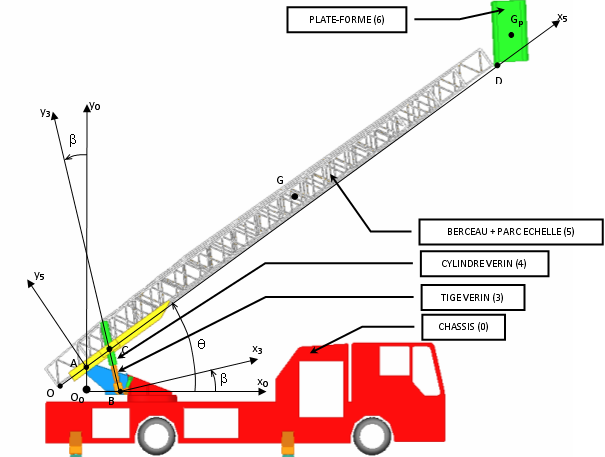
\includegraphics[width=\linewidth,keepaspectratio]{images/image5.png}Une
E.P.A.S. est une Echelle Pivotante Automatique à commande Séquentielle.
Ce système conçu et commercialisé par la société CAMIVA est monté sur le
châssis d'un camion de pompiers et permet de déplacer une plate-forme
pouvant recevoir deux personnes et un brancard le plus rapidement
possible et en toute sécurité

La course minimale du vérin de dressage pour pouvoir passer de la
position basse de l'échelle (θ=10°) à la position haute (θ=50°).

\includesvg[width=6.61111in,height=4.05208in]{images/image7.svg}

\textbf{Comment trouver la course du vérin à partir des positions
extrêmes de l'échelle~?}

\subsubsection[Cas n°2~: Détermination de l'espace de travail d'un
robot]{\texorpdfstring{\protect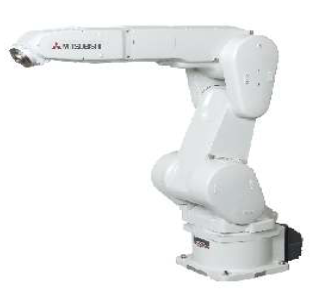
\includegraphics[width=\linewidth,keepaspectratio]{images/image8.png}Cas
n°2~: Détermination de l'espace de travail d'un
robot}{Cas n°2~: Détermination de l'espace de travail d'un robot}}\label{cas-n2-duxe9termination-de-lespace-de-travail-dun-robot}

Le robot porte-instrument est un type de robot médical. Qu'il s'agisse
d'une aiguille, d'une\\
sonde ou d'un endoscope, l'idée de ce genre de robots est d'aider le
praticien pour une\\
opération en portant l'instrument a sa place. C'est d'ailleurs à l'aide
d'un robot industriel\\
anthropomorphe que la première application chirurgicale robotisée a eu
lieu en 1985\\
pour effectuer une opération de neurochirurgie.

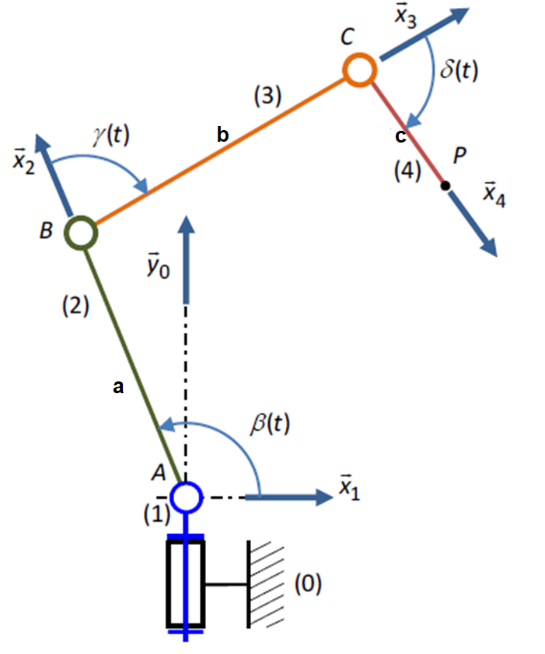
\includegraphics[width=\linewidth,keepaspectratio]{images/image9.png}

\textbf{Il est essentiel pour faire des opérations précises de connaître
ce qu'on appelle l'espace de travail, c'est-à-dire l'ensemble des
positions atteignables par le robot.}

\subsubsection{Cas n°3~: Détermination de la cylindrée d'un
micromoteur}\label{cas-n3-duxe9termination-de-la-cylindruxe9e-dun-micromoteur}


\includegraphics[width=\linewidth,keepaspectratio]{images/image10.png}Le
moteur étudié est destiné à être assemblé sur des avions de modélisme
afin de les propulser. Le moteur permet de faire tourner l'hélice à
partir de carburant (énergie thermique) situé dans un réservoir et
délivrée par un carburateur (pré actionneur). Les gazs d'échappement
s'évacuent par le pot d'échappement muni d'un silencieux.

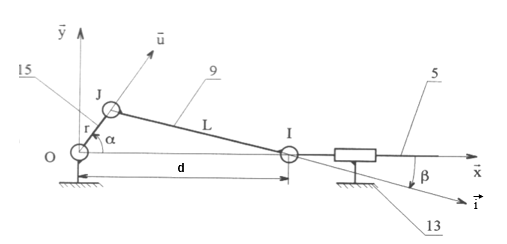
\includegraphics[width=\linewidth,keepaspectratio]{images/image11.png}\includesvg[width=6.90139in,height=2.76389in]{images/image13.svg}

Voici un extrait de la notice constructeur du moteur ENIA étudié~:

\begin{longtable}[]{@{}
  >{\raggedright\arraybackslash}p{(\columnwidth - 8\tabcolsep) * \real{0.1733}}
  >{\raggedright\arraybackslash}p{(\columnwidth - 8\tabcolsep) * \real{0.1738}}
  >{\raggedright\arraybackslash}p{(\columnwidth - 8\tabcolsep) * \real{0.2462}}
  >{\raggedright\arraybackslash}p{(\columnwidth - 8\tabcolsep) * \real{0.2468}}
  >{\raggedright\arraybackslash}p{(\columnwidth - 8\tabcolsep) * \real{0.1599}}@{}}
\toprule\noalign{}
\endhead
\bottomrule\noalign{}
\endlastfoot
\textbf{Type} & \textbf{Ø\textsubscript{piston} (mm)} &
\textbf{Cylindrée} (cm\textsuperscript{3}) & \textbf{Vitesse} (tr/min) &
\textbf{Puissance} \\
ENIA -- 32K-C & 24 & 10 & 2000-18000 & 1,2 KW \\
\end{longtable}

\textbf{Comment dimensionner le mécanisme pour obtenir la cylindrée
souhaitée~?}

En phase de conception d'un mécanisme, il faut déterminer une relation
entre le(s) mouvement(s) d'entrée et de sortie pour connaitre l'espace
de travail.

'\,'

\subsection{MODELE GEOMETRIQUE DE STRUCTURES
FERMEES}\label{modele-geometrique-de-structures-fermees}

Un mécanisme peut former une structure porteuse, mais aussi, dans bien
des cas, servir à \textbf{transformer le mouvement} et les
\textbf{efforts} pour les adapter au besoin. On parle alors de
\textbf{transmetteur}. Ces transmetteurs peuvent ainsi transformer un
mouvement continu de rotation, en mouvement alternatif de rotation ou de
translation.

L'objectif est de déterminer, par exploitation d'un modèle cinématique,
la relation mathématique caractérisant le comportement cinématique de
ces \textbf{mécanismes} utilisés comme transmetteurs ; relation appelée
\textbf{loi entrée-sortie cinématique} en \textbf{position}.

La loi \textbf{d'entrée-sortie cinématique en position} est la
\textbf{relation mathématique} reliant les paramètres de position
\textbf{d'entrée} et de \textbf{sortie}.

Dans un mécanisme transmetteur, on peut distinguer un \textbf{paramètre}
de position \textbf{d'entrée} et un \textbf{paramètre} de position de
\textbf{sortie}.

\textbf{Exemple} : dispositif bielle-manivelle

Ce mécanisme correspond à celui que l'on retrouve dans un moteur
thermique, par exemple.

Le modèle cinématique comprend 4 liaisons, 4 DDL de liaison associés à 4
paramètres de position.

Les paramètres d'entrée et de sortie sont ceux associés à la liaison
pivot L\textsubscript{01} et à la liaison

glissière L\textsubscript{30}. Pour un compresseur, l'entrée est l'angle
\(\alpha\), pour un moteur à combustion interne, l'entrée est la
distance \emph{x}.


\includegraphics[width=\linewidth,keepaspectratio]{images/image16.png}

\textbf{Exemple :} dans le cas du dispositif bielle-manivelle, la loi
entrée- sortie en position est : \(\alpha(t) = f(x(t))\)

Pour alléger écriture, la variable temporelle est rarement écrite
explicitement. Au lieu de \(\alpha(t) = f(x(t))\), on écrit plus souvent
\(\alpha = f(x)\)

\begin{longtable}[]{@{}
  >{\raggedright\arraybackslash}p{(\columnwidth - 2\tabcolsep) * \real{0.1227}}
  >{\raggedright\arraybackslash}p{(\columnwidth - 2\tabcolsep) * \real{0.8773}}@{}}
\toprule\noalign{}
\begin{minipage}[b]{\linewidth}\raggedright
\begin{quote}

\includegraphics[width=\linewidth,keepaspectratio]{images/image22.png}
\end{quote}
\end{minipage} & \begin{minipage}[b]{\linewidth}\raggedright
\textbf{Cas n°3~: Micromoteur d'avion}

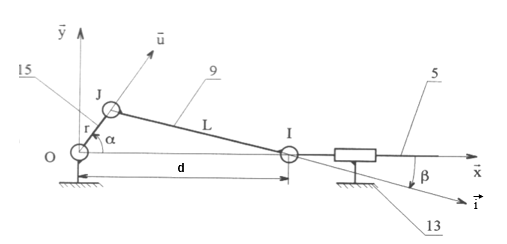
\includegraphics[width=\linewidth,keepaspectratio]{images/image11.png}

\begin{enumerate}
\def\labelenumi{\arabic{enumi}.}
\item
  Donner le mouvement d'entrée et le mouvement de sortie du micromoteur.
\item
  Identifier les paramètres de mouvement associés.
\item
  Déterminer la relation entre le paramètre de mouvement d'entrée et le
  paramètre de mouvement de sortie.
\end{enumerate}
\end{minipage} \\
\midrule\noalign{}
\endhead
\bottomrule\noalign{}
\endlastfoot
\end{longtable}

\textbf{Course}~: c'est la distance maximale parcourue par un piston
dans son cylindre, obtenue par la différence entre les deux positions
extrêmes. Pour un moteur, cela correspond à la distance parcourue par le
piston entre le point mort haut et le point mort bas.

\emph{Source : ISO 15288.}

\textbf{Définition}

\textbf{Cylindrée}~: la cylindrée est égale au volume balayé par un
piston sur sa course, multiplié par le nombre de cylindres que possède
le moteur.

\textbf{Définition}

\textbf{Homocinétique}: un mécanisme homocinétique est un mécanisme dont
la vitesse d'entrée et la vitesse de sortie sont égales (rapport de
réduction unitaire).

\textbf{Définition}


\includegraphics[width=\linewidth,keepaspectratio]{images/image24.png}\textbf{Exemples}~:
un store avec un cardan n'est pas homocinétique, alors qu'un mécanisme
avec deux cardans est homocinétique

\begin{longtable}[]{@{}
  >{\raggedright\arraybackslash}p{(\columnwidth - 2\tabcolsep) * \real{0.1227}}
  >{\raggedright\arraybackslash}p{(\columnwidth - 2\tabcolsep) * \real{0.8773}}@{}}
\toprule\noalign{}
\begin{minipage}[b]{\linewidth}\raggedright
\begin{quote}

\includegraphics[width=\linewidth,keepaspectratio]{images/image22.png}
\end{quote}
\end{minipage} & \begin{minipage}[b]{\linewidth}\raggedright
\textbf{Cas n°3~: Micromoteur d'avion}

\begin{quote}
\textbf{La loi entrée-sortie précédente peut-être représentée sous forme
graphique~:}
\end{quote}


\includegraphics{images/image25.png}

\begin{enumerate}
\def\labelenumi{\arabic{enumi}.}
\setcounter{enumi}{3}
\item
  Déterminer la course du piston.
\item
  Vérifier la cylindrée annoncée par le constructeur.
\end{enumerate}
\end{minipage} \\
\midrule\noalign{}
\endhead
\bottomrule\noalign{}
\endlastfoot
\begin{minipage}[t]{\linewidth}\raggedright
\begin{quote}
.
\end{quote}
\end{minipage} & \\
\end{longtable}

\subsection{~MODELES GEOMETRIQUES DE STRUCTURES
OUVERTES}\label{modeles-geometriques-de-structures-ouvertes}

\subsubsection[Coordonnées opérationnelles et
articulaires]{\texorpdfstring{\protect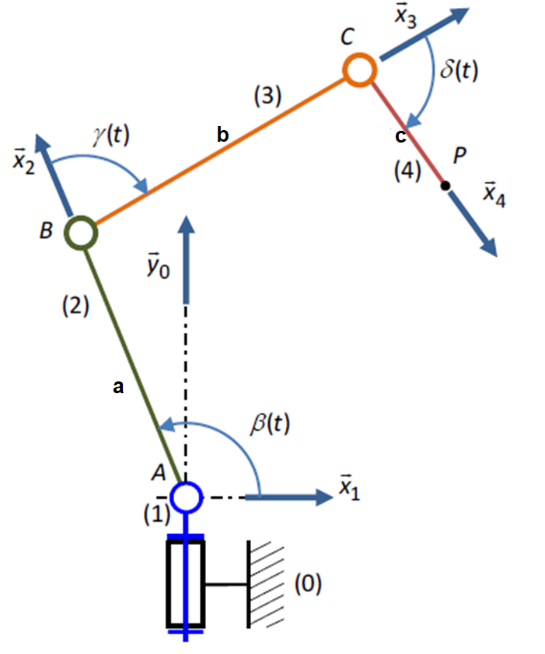
\includegraphics[width=\linewidth,keepaspectratio]{images/image9.png}Coordonnées
opérationnelles et
articulaires}{Coordonnées opérationnelles et articulaires}}\label{coordonnuxe9es-opuxe9rationnelles-et-articulaires}

Considérons le modèle cinématique d'un \textbf{robot série} à 4 degrés
de liberté tel qu'il est défini ci-contre.

L'ensemble de référence est noté (0), associé au repère
\(R_{0}(O,\overrightarrow{x_{0}},\overrightarrow{y_{0}},\overrightarrow{z_{0}})\).

L'outil est l'ensemble (4). Seule la position du point \emph{P} est
supposée fonctionnelle.

Les \textbf{coordonnées opérationnelles} sont les coordonnées de l'outil
(effecteur du mécanisme) dans le repère de référence.

Les \textbf{coordonnées articulaires} sont les paramètres de position
des liaisons du mécanisme, paramètres associés aux actionneurs (moteurs
et vérins).

Dans l'exemple, \textbf{les coordonnées opérationnelles} sont celles du
point \(P\) dans \(R_{0}\) , notées \((x,y,z)\) en posant
\(\overrightarrow{AP} = x\overrightarrow{x_{0}} + y\overrightarrow{y_{0}} + z\overrightarrow{z_{0}}\ .\ \)Les
coordonnées articulaires sont le n-uplet
(\(\alpha,\beta,\ \gamma,\ \delta\)).

En \textbf{robotique, le modèle géométrique direct} est l'ensemble des
équations permettant de calculer les coordonnées opérationnelles
(position de l'effecteur) en fonction des coordonnées articulaires.

Il faut donc trouver les coordonnées du vecteur ~\(\overrightarrow{AP}\)
dans la base
\(B_{0}(\overrightarrow{x_{0}},\overrightarrow{y_{0}},\overrightarrow{z_{0}})\).

\begin{longtable}[]{@{}
  >{\raggedright\arraybackslash}p{(\columnwidth - 2\tabcolsep) * \real{0.1226}}
  >{\raggedright\arraybackslash}p{(\columnwidth - 2\tabcolsep) * \real{0.8774}}@{}}
\toprule\noalign{}
\begin{minipage}[b]{\linewidth}\raggedright
\begin{quote}

\includegraphics[width=\linewidth,keepaspectratio]{images/image22.png}
\end{quote}
\end{minipage} & \begin{minipage}[b]{\linewidth}\raggedright
\textbf{Cas n°2~: Robot série}

\begin{enumerate}
\def\labelenumi{\arabic{enumi}.}
\item
  Donner les coordonnées opérationnelles du robot
\end{enumerate}
\end{minipage} \\
\midrule\noalign{}
\endhead
\bottomrule\noalign{}
\endlastfoot
\end{longtable}

\subsection{Rappels sur les vecteurs}\label{rappels-sur-les-vecteurs}

\subsubsection[Représentation et
définitions]{\texorpdfstring{\protect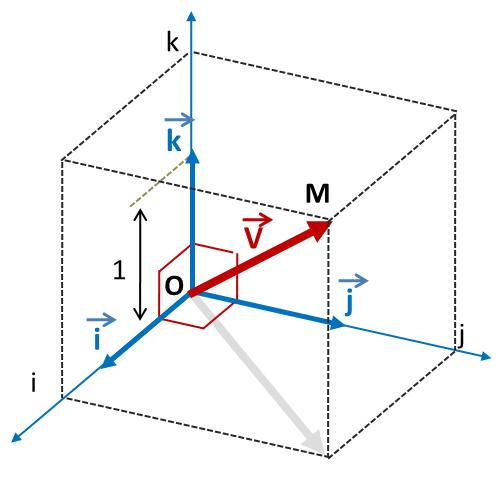
\includegraphics[width=\linewidth,keepaspectratio]{images/image26.jpeg}Représentation
et
définitions}{Représentation et définitions}}\label{repruxe9sentation-et-duxe9finitions}

Un vecteur \(\overrightarrow{V} = \overrightarrow{OM}\), représenté par
une flèche qui va du point \(O\) vers le point \(M\), est défini par ses
composantes dans la base
(\(\overrightarrow{i},\overrightarrow{j},\overrightarrow{k}\))~:

\(\overrightarrow{V} = \overrightarrow{OM} = \text{a.}\overrightarrow{\text{i}} + \text{b.}\overrightarrow{\text{j}} + \text{c.}\overrightarrow{\text{k}}\)
ou en écriture «~colonne~» \(\overrightarrow{V}\begin{pmatrix}
a \\
b \\
c
\end{pmatrix}_{(\overrightarrow{i}\text{,}\overrightarrow{\text{j}}\text{,}\overrightarrow{\text{k}})}\)

La \textbf{norme} d'un vecteur est la distance entre l'origine et
l'extrémité de ce vecteur. Elle est notée~:
\(\left\| \overrightarrow{V} \right\| = \left\| \overrightarrow{\text{OM}} \right\| = \overline{OM} = V = \ \sqrt{a^{2} + b^{2} + c^{2}}\)

\begin{longtable}[]{@{}
  >{\raggedright\arraybackslash}p{(\columnwidth - 2\tabcolsep) * \real{0.1227}}
  >{\raggedright\arraybackslash}p{(\columnwidth - 2\tabcolsep) * \real{0.8773}}@{}}
\toprule\noalign{}
\begin{minipage}[b]{\linewidth}\raggedright
\begin{quote}

\includegraphics[width=\linewidth,keepaspectratio]{images/image22.png}
\end{quote}
\end{minipage} & \begin{minipage}[b]{\linewidth}\raggedright
\begin{enumerate}
\def\labelenumi{\arabic{enumi}.}
\item
  Exprimer les coordonnées et normes des vecteurs représentés
  ci-dessous.
\end{enumerate}


\includegraphics[width=\linewidth,keepaspectratio]{images/image27.png}

\begin{enumerate}
\def\labelenumi{\arabic{enumi}.}
\setcounter{enumi}{1}
\item
  Compléter la base orthonormée directe
  \((\overrightarrow{i},\overrightarrow{j},\overrightarrow{k})\) puis
  donner les coordonnées du vecteur~\(\overrightarrow{U}\) de norme
  \(\left\| \overrightarrow{U} \right\| = U\) :
\end{enumerate}

i


\includegraphics{images/image28.png}


\includegraphics{images/image29.png}
\end{minipage} \\
\midrule\noalign{}
\endhead
\bottomrule\noalign{}
\endlastfoot
\end{longtable}

\subsubsection{Opérations sur les
vecteurs}\label{opuxe9rations-sur-les-vecteurs}

\paragraph*{\texorpdfstring{\protect
\includegraphics[width=\linewidth,keepaspectratio]{images/image30.jpeg}Addition
des vecteurs}{Addition des vecteurs}}\label{addition-des-vecteurs}
\addcontentsline{toc}{paragraph}{Addition des vecteurs}

Dans l'ensemble des vecteurs, l'\textbf{addition} d'un vecteur
\({\overrightarrow{V}}_{1}\left( X_{1},Y_{1},Z_{1} \right)\) et d'un
vecteur \({\overrightarrow{V}}_{2}\left( X_{2},Y_{2},Z_{2} \right)\)est
un \textbf{vecteur} tel que :

\[\overrightarrow{\text{V1}} + \overrightarrow{\text{V2}} = (X1 + X2)\text{.}\overrightarrow{\text{i}} + (Y1 + Y2)\text{.}\overrightarrow{\text{j}} + (Z1 + Z2)\text{.}\overrightarrow{\text{k}}\]

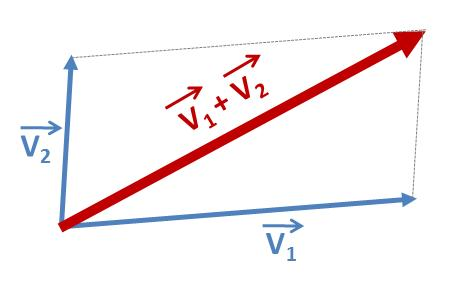
\includegraphics[width=\linewidth,keepaspectratio]{images/image31.jpeg}L'addition
vectorielle conduit à la \textbf{relation de Chasles} :
\(\overrightarrow{\text{MN}} + \overrightarrow{\text{NP}} = \overrightarrow{\text{MP}}\)

\[\overrightarrow{V1} + \overrightarrow{V2} = \begin{pmatrix}
X1 + X2 \\
Y1 + Y2 \\
Z1 + Z2
\end{pmatrix}_{(\overrightarrow{i}\text{,}\overrightarrow{\text{j}}\text{,}\overrightarrow{\text{k}})}\]

\paragraph*{Propriétés}\label{propriuxe9tuxe9s}
\addcontentsline{toc}{paragraph}{Propriétés}

\[\overrightarrow{U} + \left( \overrightarrow{V} + \overrightarrow{W} \right) = \left( \overrightarrow{U} + \overrightarrow{V} \right) + \overrightarrow{W} = \overrightarrow{U} + \overrightarrow{V} + \overrightarrow{W}\ \]

\[\overrightarrow{U} + \overrightarrow{0} = \overrightarrow{U}\]

\[\overrightarrow{U} + \overrightarrow{V} = \overrightarrow{V} + \overrightarrow{U}\]

\[\overrightarrow{U} + ( - \overrightarrow{U}) = \overrightarrow{0}\]

\paragraph*{\texorpdfstring{\protect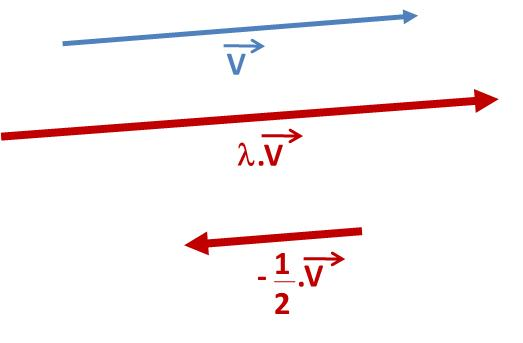
\includegraphics[width=\linewidth,keepaspectratio]{images/image32.jpeg}Multiplication
par un réel
}{Multiplication par un réel }}\label{multiplication-par-un-ruxe9el}
\addcontentsline{toc}{paragraph}{Multiplication par un réel }

Dans l'ensemble des vecteurs, la \textbf{multiplication} d'un vecteur
\(\overrightarrow{V}(X,Y,Z)\) par un \textbf{réel λ} est un
\textbf{vecteur colinéaire} à \(\overrightarrow{V}\) tel que :

\[\text{λ}\text{.}\overrightarrow{\text{V}} = \text{λ}\text{.X.}\overrightarrow{\text{i}} + \text{λ}\text{.Y.}\overrightarrow{\text{j}} + \text{λ}\text{.Z.}\overrightarrow{\text{k}}\]

\[\text{λ}\text{.}\overrightarrow{\text{V}}\begin{pmatrix}
\text{λ}\text{.X} \\
\text{λ}\text{.Y} \\
\text{λ}\text{Z}
\end{pmatrix}_{(\overrightarrow{i}\text{,}\overrightarrow{\text{j}}\text{,}\overrightarrow{\text{k}})}\]

\paragraph*{Propriétés}\label{propriuxe9tuxe9s-1}
\addcontentsline{toc}{paragraph}{Propriétés}

\[\lambda.\left( µ.\overrightarrow{U} \right) = (\lambda\mu).\overrightarrow{U}\]

\[\lambda.\left( \overrightarrow{U} + \overrightarrow{V} \right) = \lambda.\overrightarrow{U} + \lambda.\overrightarrow{V}\]

\((\lambda + µ).\overrightarrow{U} = \lambda.\overrightarrow{U} + µ.\overrightarrow{U}\)

\[1.\overrightarrow{U} = \overrightarrow{U}\]

\begin{longtable}[]{@{}
  >{\raggedright\arraybackslash}p{(\columnwidth - 2\tabcolsep) * \real{0.1227}}
  >{\raggedright\arraybackslash}p{(\columnwidth - 2\tabcolsep) * \real{0.8773}}@{}}
\toprule\noalign{}
\begin{minipage}[b]{\linewidth}\raggedright
\begin{quote}

\includegraphics[width=\linewidth,keepaspectratio]{images/image22.png}
\end{quote}
\end{minipage} & \begin{minipage}[b]{\linewidth}\raggedright
\textbf{Application~: Vitesse d'un bateau}

Une petite embarcation, dont le moteur génère une vitesse de 40 km/h,
traverse de la rive sud à la rive nord d'une rivière coulant vers l'est
avec un courant de 15 km/h. L'embarcation se dirige avec un angle de 50°
par rapport au rivage d'une rivière vers un quai situé légèrement à
l'est de son point de départ.

Quelle est la vitesse réelle de l'embarcation sachant qu'elle correspond
à l'addition vectorielle de la vitesse du bateau avec celle du courant~?
\end{minipage} \\
\midrule\noalign{}
\endhead
\bottomrule\noalign{}
\endlastfoot
& \\
\end{longtable}

\subsubsection{Produit scalaire}\label{produit-scalaire}

\paragraph*{\texorpdfstring{Définition
}{Définition }}\label{duxe9finition}
\addcontentsline{toc}{paragraph}{Définition }

Le produit scalaire des deux vecteurs \(\overrightarrow{U}\) et
\(\overrightarrow{V}\) est le \textbf{nombre réel} suivant noté
\(\overrightarrow{U} \bullet \overrightarrow{V}\):

\[\overrightarrow{U} \bullet \overrightarrow{V} = \left\| \overrightarrow{U} \right\|.\left\| \overrightarrow{V} \right\|.cos(\overrightarrow{U},\overrightarrow{V})\]

\paragraph*{\texorpdfstring{\protect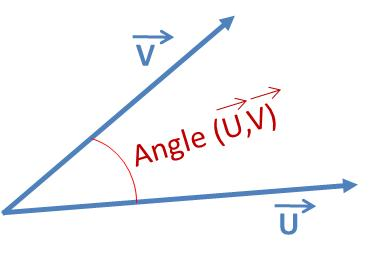
\includegraphics[width=\linewidth,keepaspectratio]{images/image33.jpeg}Expression
analytique}{Expression analytique}}\label{expression-analytique}
\addcontentsline{toc}{paragraph}{Expression analytique}

Dans une \textbf{base orthonormée}
(\(\overrightarrow{i},\overrightarrow{j},\overrightarrow{k}\)) le
produit scalaire des deux vecteurs vecteur
\({\overrightarrow{V}}_{1}\left( X_{1},Y_{1},Z_{1} \right)\) et
\({\overrightarrow{V}}_{2}\left( X_{2},Y_{2},Z_{2} \right)\) s'écrit :

\textbf{Réel}

\(\overrightarrow{V_{1}}\  \bullet \overrightarrow{V_{2}} = \text{ }\text{X}_{1}\text{. }\text{X}_{2} + Y_{1}\text{. }\text{Y}_{2} + Z_{1}\text{. }\text{Z}_{2}\)

\paragraph*{Propriétés}\label{propriuxe9tuxe9s-2}
\addcontentsline{toc}{paragraph}{Propriétés}

\emph{Symétrie :}
\(\overrightarrow{U} \bullet \overrightarrow{V} = \overrightarrow{V} \bullet \overrightarrow{U}\)

\emph{Distributivité :}
\(\overrightarrow{U} \bullet (\overrightarrow{V} + \overrightarrow{W}) = \overrightarrow{U} \bullet \overrightarrow{V} + \overrightarrow{U} \bullet \overrightarrow{W}\)

\emph{Multiplication par un réel :}
\(\lambda.\overrightarrow{U} \bullet µ.\overrightarrow{V} = \lambda µ.\overrightarrow{U} \bullet \overrightarrow{V}\)

\[\overrightarrow{U} \bullet \overrightarrow{U} = U^{2} \geq 0\]

\paragraph*{\texorpdfstring{\protect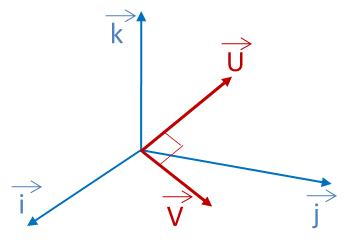
\includegraphics[width=\linewidth,keepaspectratio]{images/image34.jpeg}Cas
particulier}{Cas particulier}}\label{cas-particulier}
\addcontentsline{toc}{paragraph}{Cas particulier}

Le produit scalaire est \textbf{nul} :

\begin{itemize}
\item
  Si un des deux vecteurs est nul
\item
  Si les 2 vecteurs sont \textbf{⊥}
\end{itemize}

Dans une même base orthonormée
(\(\overrightarrow{i},\overrightarrow{j},\overrightarrow{k}\)), on a
donc \(\overrightarrow{i} \bullet \overrightarrow{i}\) =
\(\overrightarrow{j} \bullet \overrightarrow{j}\ \)=
\(\overrightarrow{k} \bullet \overrightarrow{k}\ \)= 1

et donc \(\overrightarrow{i} \bullet \overrightarrow{j}\) =
\(\overrightarrow{j} \bullet \overrightarrow{k}\ \)=
\(\overrightarrow{k} \bullet \overrightarrow{i}\) = 0

'\,'

\begin{longtable}[]{@{}
  >{\raggedright\arraybackslash}p{(\columnwidth - 2\tabcolsep) * \real{0.1227}}
  >{\raggedright\arraybackslash}p{(\columnwidth - 2\tabcolsep) * \real{0.8773}}@{}}
\toprule\noalign{}
\begin{minipage}[b]{\linewidth}\raggedright
\begin{quote}

\includegraphics[width=\linewidth,keepaspectratio]{images/image22.png}
\end{quote}
\end{minipage} & \begin{minipage}[b]{\linewidth}\raggedright
Calculer le produit scalaire
\(\overrightarrow{V_{1}} \bullet \overrightarrow{V_{2}}\) avec
\(\overrightarrow{V_{1}} = (2.\overrightarrow{x} + 2.\overrightarrow{y} - 3.\overrightarrow{z})\mspace{6mu} et\mspace{6mu}\overrightarrow{V_{2}} = ( - \overrightarrow{x} + 6.\overrightarrow{z})\)
\end{minipage} \\
\midrule\noalign{}
\endhead
\bottomrule\noalign{}
\endlastfoot
& \\
\end{longtable}

\begin{longtable}[]{@{}
  >{\raggedright\arraybackslash}p{(\columnwidth - 2\tabcolsep) * \real{0.1227}}
  >{\raggedright\arraybackslash}p{(\columnwidth - 2\tabcolsep) * \real{0.8773}}@{}}
\toprule\noalign{}
\begin{minipage}[b]{\linewidth}\raggedright
\begin{quote}

\includegraphics[width=\linewidth,keepaspectratio]{images/image22.png}
\end{quote}
\end{minipage} & \begin{minipage}[b]{\linewidth}\raggedright
Calculer les produits scalaires suivants~:

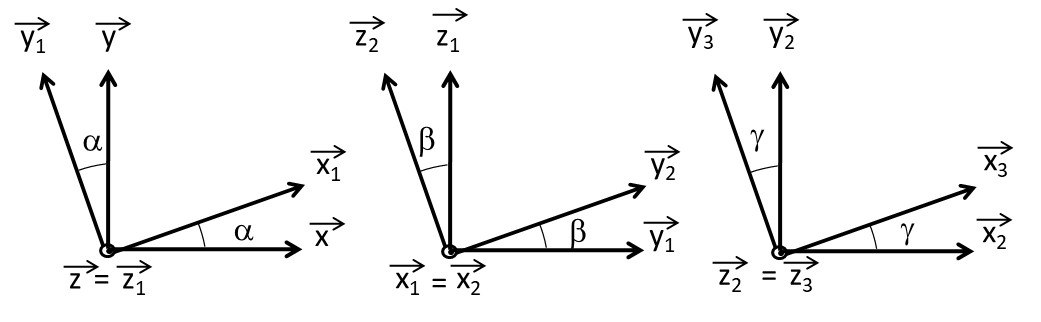
\includegraphics[width=\linewidth,keepaspectratio]{images/image35.jpeg}

\(\overrightarrow{x_{1}} \bullet \overrightarrow{x_{0}} =\)
\(\overrightarrow{x_{2}} \bullet \overrightarrow{x_{1}} =\)
\(\overrightarrow{z_{2}} \bullet \overrightarrow{x_{0}} =\)

\(\overrightarrow{y_{0}} \bullet \overrightarrow{x_{0}} =\)
\(\overrightarrow{x_{2}} \bullet \overrightarrow{x_{0}} =\)
\(\overrightarrow{z_{3}} \bullet \overrightarrow{x_{0}} =\)

\(\overrightarrow{z_{1}} \bullet \overrightarrow{x_{0}} =\)
\(\overrightarrow{y_{0}} \bullet \overrightarrow{x_{2}} =\)
\(\overrightarrow{y_{3}} \bullet \overrightarrow{z_{1}} =\)
\end{minipage} \\
\midrule\noalign{}
\endhead
\bottomrule\noalign{}
\endlastfoot
& \\
\end{longtable}

\subsubsection[Modèles géométriques direct et
inverse]{\texorpdfstring{Modèles géométriques direct et
inverse\protect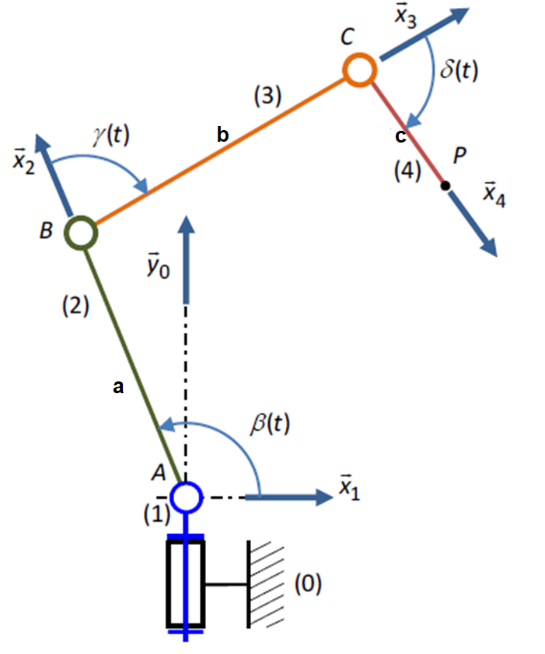
\includegraphics[width=\linewidth,keepaspectratio]{images/image9.png}}{Modèles géométriques direct et inverse}}\label{moduxe8les-guxe9omuxe9triques-direct-et-inverse}

En \textbf{robotique}, le \textbf{modèle géométrique direct} est
l'ensemble des équations permettant de calculer les \textbf{coordonnées
opérationnelles} (position de l'effecteur) en fonction des
\textbf{coordonnées articulaires}.

\begin{longtable}[]{@{}
  >{\raggedright\arraybackslash}p{(\columnwidth - 2\tabcolsep) * \real{0.1227}}
  >{\raggedright\arraybackslash}p{(\columnwidth - 2\tabcolsep) * \real{0.8773}}@{}}
\toprule\noalign{}
\begin{minipage}[b]{\linewidth}\raggedright
\begin{quote}

\includegraphics[width=\linewidth,keepaspectratio]{images/image22.png}
\end{quote}
\end{minipage} & \begin{minipage}[b]{\linewidth}\raggedright
Trouver les coordonnées opérationnelles du robot.
\end{minipage} \\
\midrule\noalign{}
\endhead
\bottomrule\noalign{}
\endlastfoot
& \\
\end{longtable}

Le \textbf{modèle géométrique inverse} permet de calculer les
coordonnées articulaires en fonction des coordonnées opérationnelles.

\begin{enumerate}
\def\labelenumi{\arabic{enumi}.}
\item
  Imposer une position ou une contrainte de position
\end{enumerate}

Pour \textbf{imposer une position} à un effecteur, il est nécessaire de
déterminer le \textbf{modèle géométrique direct puis de l'inverser}
numériquement ou en calculant le modèle géométrique indirect.

Une \textbf{contrainte de position limite les mouvements} possibles de
l'effecteur. Elle s'exprime par une ou plusieurs \textbf{expressions
vectorielles}.

Exemples :

\begin{itemize}
\item
  contrainte de \textbf{distance} = contrainte sur une \textbf{norme}
\item
  contrainte \textbf{d'appartenance} à une \textbf{droite} = contrainte
  sur 2 coordonnées
\item
  contraintes d'appartenance à un \textbf{plan} = contrainte sur une
  \textbf{coordonnée}
\item
  contrainte de \textbf{trajectoire} = contrainte sur les
  \textbf{coordonnées}.
\end{itemize}

Exemples de contraintes :

\begin{itemize}
\item
  le point \emph{P} doit rester à une distance inférieure à \emph{d} de
  son origine bâti \emph{A}, soit à l'intérieur d'une sphère de rayon
  \(d\) \(\left\| \overrightarrow{AP} \right\| \leq d\)
\item
  Le point \emph{P} doit rester à une hauteur \emph{h} du « sol », soit
  sur un plan parallèle à
  \((\overrightarrow{x_{0}},\overrightarrow{z_{0}})\)\textsubscript{~:}
  \(\overrightarrow{AP} \bullet \overrightarrow{y_{0}} = h\)
\item
  Le point \emph{P} doit se situer sur une droite verticale passant par
  le point \emph{D}(\emph{L},0,0) :
\end{itemize}

\(\overrightarrow{AP} \bullet \overrightarrow{x_{0}} = L\)~;
\(\overrightarrow{AP} \bullet \overrightarrow{y_{0}} = 0\)~;
\(\overrightarrow{AP} \bullet \overrightarrow{z_{0}} = 0\)~

\subsection{MODELE GEOMETRIQUE DE STRUCTURES
FERMEES}\label{modele-geometrique-de-structures-fermees-1}

\subsubsection{Déterminer la loi d'entrée-sortie en position par
fermeture
géométrique}\label{duxe9terminer-la-loi-dentruxe9e-sortie-en-position-par-fermeture-guxe9omuxe9trique}

Dans un mécanisme en chaîne fermée utilisé comme transmetteur, il n'y a
qu'une seule liaison « motorisée ». C'est la structure bouclée du
mécanisme qui fait que la mise en mouvement de cette liaison entraîne
celle de tout le mécanisme. Cette \textbf{structure bouclée} du
mécanisme se retrouve dans le graphe des liaisons sous la forme
\textbf{d'une chaîne fermée}.

\textbf{Démarche pour obtenir une loi entrée-sortie en position} :

\begin{enumerate}
\def\labelenumi{\arabic{enumi}.}
\item
  Identifier les paramètre de mouvement d'entrée et de sortie
\item
  Ecrire la relation vectorielle de fermeture géométrique
\item
  Projeter l'équation de fermeture dans une base choisie
\item
  Eliminer les paramètres intermédiaires en combinant les équations
  obtenues~:

  \begin{enumerate}
  \def\labelenumii{\alph{enumii}.}
  \item
    \textbf{pour éliminer un} angle on isole les termes en cosinus et
    sinus de l'angle puis on utilise \(\cos^{2} + \sin^{2} = 1\)

    \begin{enumerate}
    \def\labelenumiii{\roman{enumiii}.}
    \item
      Exemple~:
      \(\left( Rcos(\alpha) \right)^{2} + \left( Rsin(\alpha) \right)^{2} = R²\)
    \end{enumerate}
  \item
    pour éliminer une distance, on fait apparaitre la tangente

    \begin{enumerate}
    \def\labelenumiii{\roman{enumiii}.}
    \item
      Exemple~:
      \(\frac{\lambda sin(\alpha)}{\lambda cos(\alpha)} = tan(\alpha\))
    \end{enumerate}
  \end{enumerate}
\item
  Faire apparaitre la relation entre le paramètre de mouvement d'entrée
  et le paramètre de mouvement de sortie
\end{enumerate}

\textbf{Exemple avec le dispositif bielle-manivelle}


\includegraphics[width=\linewidth,keepaspectratio]{images/image16.png}

\begin{longtable}[]{@{}
  >{\raggedright\arraybackslash}p{(\columnwidth - 2\tabcolsep) * \real{0.1227}}
  >{\raggedright\arraybackslash}p{(\columnwidth - 2\tabcolsep) * \real{0.8773}}@{}}
\toprule\noalign{}
\begin{minipage}[b]{\linewidth}\raggedright
\begin{quote}

\includegraphics[width=\linewidth,keepaspectratio]{images/image22.png}
\end{quote}
\end{minipage} & \begin{minipage}[b]{\linewidth}\raggedright
\begin{enumerate}
\def\labelenumi{\arabic{enumi}.}
\item
  \textbf{Identifier le paramètre de mouvement d'entrée et le paramètre
  de mouvement de sortie}
\end{enumerate}

Entrée~: translation de 3/0, paramétrée par la distance \(x\)

Sortie~: rotation de 1/0, paramétré par l'angle \(\alpha\)

\begin{enumerate}
\def\labelenumi{\arabic{enumi}.}
\setcounter{enumi}{1}
\item
  \textbf{Ecrire la relation vectorielle de fermeture géométrique}
\end{enumerate}

\[\overrightarrow{AB} + \overrightarrow{BC} + \ldots + \overrightarrow{DA} = \overrightarrow{0}\]

\[\overrightarrow{AB} + \overrightarrow{BC} + \overrightarrow{CA} = \overrightarrow{0}\]

\[e\ \overrightarrow{x_{1}} + \ L\ \overrightarrow{x_{2}} - x\ \overrightarrow{x_{0}} = \overrightarrow{0}\]

\begin{enumerate}
\def\labelenumi{\arabic{enumi}.}
\setcounter{enumi}{2}
\item
  Projeter l'équation dans la base de référence (en général, la
  \textbf{base de référence - i.e celle du bâti}).
\end{enumerate}

\[\left\{ \begin{array}{r}
\ \ /\overrightarrow{x_{0}}\ \ \ \ \ \ \ \ e\ \overrightarrow{x_{1}} \bullet \overrightarrow{x_{0}} + \ L\ \overrightarrow{x_{2}} \bullet \overrightarrow{x_{0}} - x\ \overrightarrow{x_{0}} \bullet \overrightarrow{x_{0}} = \overrightarrow{0} \bullet \overrightarrow{x_{0}} \\
/\overrightarrow{y_{0}}\ \ \ \ e\ \overrightarrow{x_{1}} \bullet \overrightarrow{y_{0}} + \ L\ \overrightarrow{x_{2}} \bullet \overrightarrow{y_{0}} - x\ \overrightarrow{x_{0}} \bullet \overrightarrow{y_{0}} = \overrightarrow{0} \bullet \overrightarrow{y_{0}}
\end{array} \right.\ \ \ \ \ \ \ \ \ \ \ \ \]

\[\left\{ \begin{array}{r}
\ \ /\overrightarrow{x_{0}}\ \ \ \ \ \ \ \ e\ \cos(\alpha) + \ L\ \cos(\beta) - x\  = 0 \\
/\overrightarrow{y_{0}}\ \ \ \ e\ \sin(\alpha) + \ L\ \sin(\beta) = 0
\end{array} \right.\ \ \ \ \ \ \ \ \ \ \ \ \]

On obtient donc deux équations pour un modèle plan ou trois équations
scalaires pour un modèle spatial~:

\begin{enumerate}
\def\labelenumi{\arabic{enumi}.}
\setcounter{enumi}{3}
\item
  \textbf{Eliminer les paramètres intermédiaires} en combinant les
  équations obtenues~:
\end{enumerate}

\begin{itemize}
\item
  \textbf{pour éliminer un angle} on isole les termes en cosinus et
  sinus de l'angle puis on utilise \(\cos^{2} + \sin^{2} = 1\)
\end{itemize}

\[\left\{ \begin{array}{r}
L\ cos(\beta) = x - {e\ cos}{(\alpha)\ \ (1)} \\
L\ sin(\beta) = - e\ \sin(\alpha)\ \ \ \ \ \ (2)
\end{array} \right.\ \]

\[{(1)}^{2} + {(2)}^{2} \rightarrow L^{2}\ \cos^{2}(\beta)\  + \ L^{2}\ \sin^{2}(\beta) = \left( x - {e\ cos}(\alpha) \right)^{2} + \left( - e\ \sin(\alpha) \right)^{2}\]

\[L^{2}\  = \left( x - {e\ cos}(\alpha) \right)^{2} + \left( - e\ \sin(\alpha) \right)^{2}\]

\begin{itemize}
\item
  \textbf{pour éliminer une distance}, on fait apparaitre la tangente~:
\end{itemize}

\[\left\{ \begin{array}{r}
L\ cos(\beta) = x - {e\ cos}{(\alpha)\ \ (1)} \\
L\ sin(\beta) = - e\ \sin(\alpha)\ \ \ \ \ \ (2)
\end{array} \right.\ \]

\[\frac{(2)}{(1)} \rightarrow \frac{L\ sin(\beta)}{L\ cos(\beta)} = \frac{- e\ \sin(\alpha)}{x - {e\ cos}(\alpha)}\]

\[\tan(\beta) = \frac{e\ \sin(\alpha)}{{e\ cos}{(\alpha) - x}}\]
\end{minipage} \\
\midrule\noalign{}
\endhead
\bottomrule\noalign{}
\endlastfoot
\end{longtable}

\paragraph*{Deuxième méthode}\label{deuxiuxe8me-muxe9thode}
\addcontentsline{toc}{paragraph}{Deuxième méthode}

Il existe une autre méthode qui consiste à écrire la norme au carré d'un
des termes de la fermeture géométrique (en général celui qu'on isole).

\[\left\| \overrightarrow{AE} \right\|^{2} = {(\overrightarrow{AB} + \overrightarrow{BC} + \ldots + \overrightarrow{DE})}^{2} = {\overrightarrow{AB}}^{2} + \ldots + {\overrightarrow{DE}}^{2} + 2\overrightarrow{AB} \bullet \overrightarrow{BC} + \ldots + 2\overrightarrow{CD} \bullet \overrightarrow{DE}\]

\[e\ \overrightarrow{x_{1}} + \ L\ \overrightarrow{x_{2}} - x\ \overrightarrow{x_{0}} = \overrightarrow{0}\]

\[\ L\ \overrightarrow{x_{2}} = x\ \overrightarrow{x_{0}} - e\ \overrightarrow{x_{1}}\]

\[\left( \ L\ \overrightarrow{x_{2}} \right)^{2} = \left( x\ \overrightarrow{x_{0}} - e\ \overrightarrow{x_{1}} \right)^{2}\]

\[L^{2} = x^{2} - 2ex\ {\overrightarrow{x_{0}} \bullet \overrightarrow{x_{1}} + e}^{2}\]

\[L^{2} = x^{2}{+ e}^{2} - 2excos(\alpha)\ \]

\paragraph*{Troisième méthode}\label{troisiuxe8me-muxe9thode}
\addcontentsline{toc}{paragraph}{Troisième méthode}

Enfin, lorsque le mécanisme est sous forme d'un triangle quelconque
(typiquement un dispositif bielle-manivelle), le théorème d'Al-Kashi
peut être avantageusement utilisé. Dans ce cas-là la relation est
directement obtenue~:

\[L^{2} = x^{2}{+ e}^{2} - 2excos(\alpha)\ \]


\includegraphics[width=\linewidth,keepaspectratio]{images/image16.png}

\paragraph*{Quatrième méthode}\label{quatriuxe8me-muxe9thode}
\addcontentsline{toc}{paragraph}{Quatrième méthode}

Parfois on utilise l'orthogonalité de deux vecteurs pour déterminer la
loi entrée-sortie, voir l'exercice sur la barrière sinusmatic.

\begin{longtable}[]{@{}
  >{\raggedright\arraybackslash}p{(\columnwidth - 2\tabcolsep) * \real{0.1226}}
  >{\raggedright\arraybackslash}p{(\columnwidth - 2\tabcolsep) * \real{0.8774}}@{}}
\toprule\noalign{}
\begin{minipage}[b]{\linewidth}\raggedright
\begin{quote}

\includegraphics[width=\linewidth,keepaspectratio]{images/image22.png}
\end{quote}
\end{minipage} & \begin{minipage}[b]{\linewidth}\raggedright
\textbf{Cas n°1 : Echelle EPAS}

La course minimale du vérin de dressage pour pouvoir passer de la
position basse de l'échelle (θ=10°) à la position haute (θ=50°).

avec \(\overline{O_{0}A} = a\) ; \(\overline{AC} = c\)~;
\(\overline{O_{0}B} = b\)~; \(\overline{BC} = r(t)\)

\includesvg[width=5.36111in,height=3.28542in]{images/image7.svg}

\begin{enumerate}
\def\labelenumi{\arabic{enumi}.}
\item
  Déterminer la loi entrée-sortie.
\item
  Déterminer la course du vérin pour obtenir les mouvements souhaités.
\end{enumerate}

\emph{On prendra c=2,6m~; a=2m, b=3m}
\end{minipage} \\
\midrule\noalign{}
\endhead
\bottomrule\noalign{}
\endlastfoot
\end{longtable}

\subsection{LOI ENTREE SORTIE EN
VITESSE}\label{loi-entree-sortie-en-vitesse}

\begin{quote}
On appelle \textbf{loi entrée-sortie en en vitesse} d'un mécanisme, la
\textbf{relation} mathématique entre la \textbf{dérivée temporelle} du
\textbf{paramètre de position} du \textbf{solide d'entrée}, et celle du
\textbf{solide de sortie}.
\end{quote}

L'objectif étant d'anticiper les effets, sur le solide de sortie, du
mouvement imposé au solide en entrée, ces relations ne doivent pas faire
intervenir les paramètres de mouvement des liaisons internes au
mécanisme.

Après pris soin de bien identifié les paramètres d'entrée et de sortie,
les méthodes pour obtenir une loi entrée- sortie cinématiques sont :

\begin{longtable}[]{@{}
  >{\raggedright\arraybackslash}p{(\columnwidth - 4\tabcolsep) * \real{0.3264}}
  >{\raggedright\arraybackslash}p{(\columnwidth - 4\tabcolsep) * \real{0.2883}}
  >{\raggedright\arraybackslash}p{(\columnwidth - 4\tabcolsep) * \real{0.3852}}@{}}
\toprule\noalign{}
\begin{minipage}[b]{\linewidth}\raggedright
\textbf{Fermeture géométrique}
\end{minipage} & \begin{minipage}[b]{\linewidth}\raggedright
\end{minipage} & \begin{minipage}[b]{\linewidth}\raggedright
\end{minipage} \\
\midrule\noalign{}
\endhead
\bottomrule\noalign{}
\endlastfoot
\begin{minipage}[t]{\linewidth}\raggedright
\begin{quote}
Loi entrée-sortie \textbf{en position}
\end{quote}
\end{minipage} & Dérivation &
\begin{minipage}[t]{\linewidth}\raggedright
\begin{quote}
Loi entrée-sortie \textbf{en vitesse}
\end{quote}
\end{minipage} \\
\end{longtable}

\begin{longtable}[]{@{}
  >{\raggedright\arraybackslash}p{(\columnwidth - 4\tabcolsep) * \real{0.3264}}
  >{\raggedright\arraybackslash}p{(\columnwidth - 4\tabcolsep) * \real{0.2883}}
  >{\raggedright\arraybackslash}p{(\columnwidth - 4\tabcolsep) * \real{0.3852}}@{}}
\toprule\noalign{}
\begin{minipage}[b]{\linewidth}\raggedright
\textbf{Fermeture cinématique}
\end{minipage} & \begin{minipage}[b]{\linewidth}\raggedright
\end{minipage} & \begin{minipage}[b]{\linewidth}\raggedright
Loi entrée-sortie \textbf{en vitesse}
\end{minipage} \\
\midrule\noalign{}
\endhead
\bottomrule\noalign{}
\endlastfoot
\end{longtable}

Lorsqu'on dérive les fonctions trigonométriques~:
\(\frac{dsin(\alpha)}{dt} = \dot{\alpha}cos(\alpha)\)

\subsection{Sources}\label{sources}

Ce cours a été élaboré à l'aide de nombreuses ressources~provenant de
documents publics d'industriels, des activités pédagogiques de collègues
de l'UPSTI.

\subsection{Exercices du chapitre}\label{exercices-du-chapitre}


\includegraphics[width=\linewidth,keepaspectratio]{images/image36.png}


\includegraphics[width=\linewidth,keepaspectratio]{images/image38.png}\textbf{SYSTÈME
D'ORIENTATION D'ANTENNE}


\includegraphics[width=\linewidth,keepaspectratio]{images/image37.png}
Niveau 1

\emph{(\ul{Source :} Jérôme Letard)}

\textbf{\ul{Objectifs de l'étude~:}}

\begin{itemize}
\item
  \textbf{Réaliser} le schéma cinématique du système d'orientation
  d'antenne.
\item
  \textbf{Déterminer} la durée d'alimentation du vérin électrique du
  système d'orientation d'antenne pour un déplacement donné.

  \begin{enumerate}
  \item
    
\includegraphics[width=\linewidth,keepaspectratio]{images/image39.png}Mise
    en situation
  \end{enumerate}
\end{itemize}

x\textsubscript{0}

y\textsubscript{0}


\includegraphics[width=\linewidth,keepaspectratio]{images/image40.png}Le
système d'orientation d'antenne ci-contre permet, grâce à une
télécommande, de régler à distance l'orientation de sa parabole afin
d'optimiser la réception des chaines de télévision.

Pour cela, le moteur du vérin électrique (type~: vis/écrou --
p\textsubscript{vis} = 2 mm/tr)) est alimenté, de façon à faire rentrer
ou sortir la tige et obtenir ainsi la position de l'antenne désirée.

La modélisation du système d'antenne est la suivante~:

\textbf{A}

\textbf{B}

\textbf{C}

α\textsubscript{1}

α\textsubscript{2}

d

\[\overrightarrow{AC} = l_{0}.{\overrightarrow{x}}_{0},\overline{AB} = l_{1}\]

\begin{enumerate}
\def\labelenumi{\arabic{enumi}.}
\item
  \textbf{Déterminer} la loi entrée sortie du mécanisme.
\end{enumerate}


\includegraphics[width=\linewidth,keepaspectratio]{images/image57.png}\textbf{ÉTUDE
DU PHR DE L'AIRBUS A340}


\includegraphics[width=\linewidth,keepaspectratio]{images/image37.png}
Niveau 2

\emph{(\ul{Source :} CCP MP 2005)}

\textbf{\ul{Objectif de l'étude~:}}

\begin{itemize}
\item
  \textbf{Déterminer} la longueur utile de la vis du dispositif de
  commande du PHR.
\end{itemize}


\includegraphics[width=\linewidth,keepaspectratio]{images/image58.jpeg}L'empennage
horizontal, ou Plan Horizontal Réglable (PHR), peut être assimilé à une
mini aile située à l'extrémité du fuselage de l'avion. Il a pour objet
de stabiliser l\textquotesingle avion en l\textquotesingle empêchant de
pivoter autour de son centre de gravité.

\textbf{Empennage horizontal}


\includegraphics[width=\linewidth,keepaspectratio]{images/image59.jpeg}

Le PHR est actionné par la vis de manœuvre \textbf{4}, représentée sur
les figures suivantes par le segment RH où elle est considérée comme un
élément déformable de raideur k. L'action sur cette vis va faire pivoter
le PHR d'un angle β.

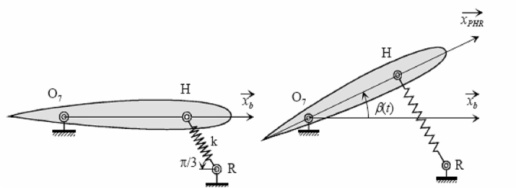
\includegraphics[width=\linewidth,keepaspectratio]{images/image60.jpeg}Afin
de répondre aux exigences de fiabilité qui stipulent, en particulier,
que le PHR doit pouvoir fonctionner durant 10\textsuperscript{9} FH (Fly
Hour) sans subir de défaillance, un certain nombre de composants de la
chaîne de commande du PHR sont doublés ou triplés suivant les cas.

D'autre part, toujours par souci de sécurité, le PHR peut être
commandé~:

\begin{itemize}
\item
  soit automatiquement par un ordinateur de bord qui détermine, à partir
  des paramètres du vol, la valeur optimale de l'angle \emph{β},
\item
  soit manuellement par le pilote à partir d'un volant de commande situé
  dans le poste de pilotage et ce en cas de défaillance de la commande
  automatique du PHR.
\end{itemize}


\includegraphics[width=\linewidth,keepaspectratio]{images/image61.jpeg}

Dans les deux cas, les consignes émises par le calculateur ou par le
pilote agissent sur les tiroirs des distributeurs alimentant deux
moteurs hydrauliques fonctionnant simultanément et dont les arbres de
sortie entraînent, via un différentiel et un réducteur, la rotation de
la vis \textbf{4} et donc celle du PHR.

En raison de sa complexité, on se limitera, dans le cadre de ce sujet, à
une étude «~simplifiée~» de l'asservissement en position angulaire de la
vis \textbf{4} agissant sur le PHR.

La figure ci-contre présente globalement la situation des différents
éléments intervenant dans cette étude~: les moteurs hydrauliques, le
différentiel, les distributeurs, les moteurs électriques (au nombre de
trois par sécurité, mais un seul fonctionne à un instant donné), la vis
\textbf{4}.

Le schéma de principe de commande de la vis \textbf{4} ainsi que son
asservissement sont présentés
ci-après.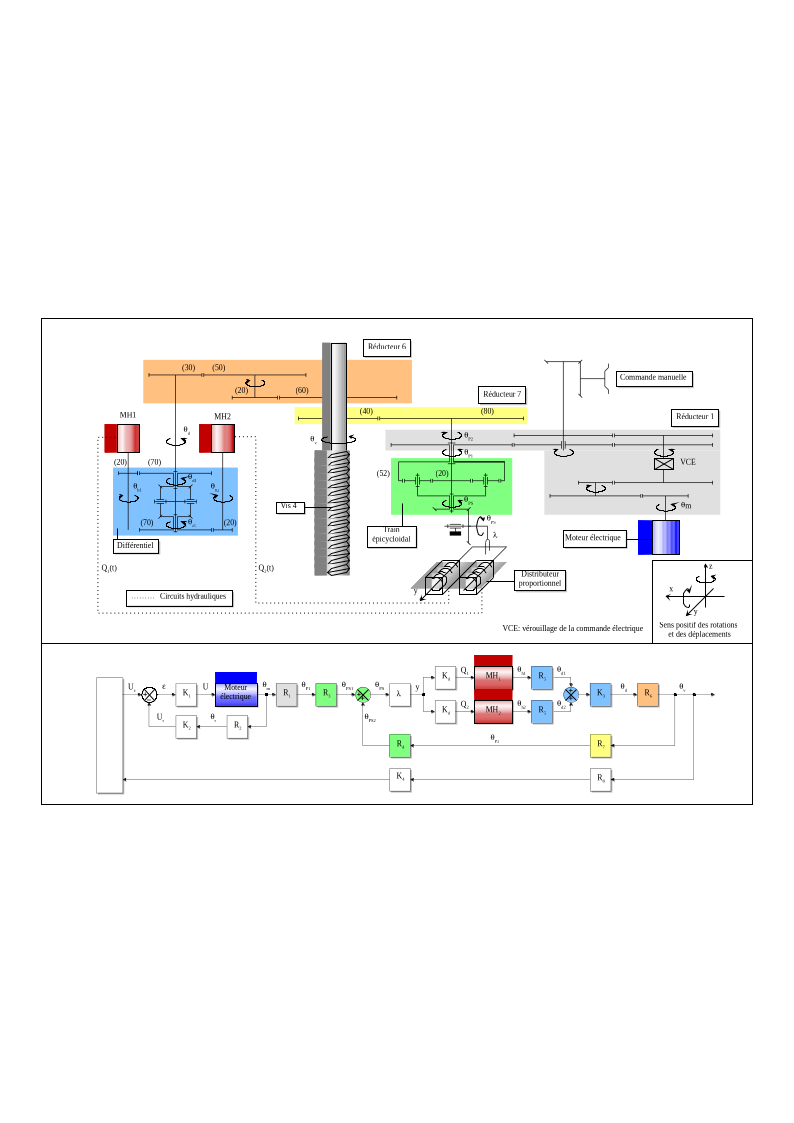
\includegraphics[width=\linewidth,keepaspectratio]{images/image62.png}

\begin{enumerate}
\item
  Dispositif de commande mécanique du PHR
\end{enumerate}

Les moteurs hydrauliques manœuvrent la vis \textbf{4} par
l'intermédiaire d'un réducteur à engrenage. Cette vis est reliée à la
structure avion \textbf{1} par l'intermédiaire d'une suspension à
CARDAN, c\textquotesingle est-à-dire que la pièce \textbf{3} est reliée
par deux liaisons pivots en série, d'axes orthogonaux, à la structure
\textbf{1}.

L'écrou \textbf{5} entraîne l'équerre \textbf{7}, solidaire du PHR, par
l'intermédiaire d'une autre suspension à CARDAN. Le PHR est lié à
\textbf{1} par l'intermédiaire d'une liaison pivot.


\includegraphics[width=\linewidth,keepaspectratio]{images/image63.png}

\textbf{\ul{Schéma cinématique du dispositif de commande du PHR}}
(
\includegraphics{images/image64.png})

Dans l'objectif de déterminer la longueur utile de la vis \textbf{4}, on
souhaite établir la loi entrée/sortie du dispositif de commande du PHR.

Pour cela on utilisera une modèle simplifié du système. On ne tient pas
compte des suspensions à CARDAN~: On remplace la liaison pivot entre
\textbf{2} et \textbf{3} ainsi que la liaison pivot entre \textbf{5} et
\textbf{6} par des liaisons encastrement.

\emph{\ul{Données~:}}

\(O_{4}H = z(t)\) \emph{(que l'on notera}

\includegraphics{images/image65.png}\emph{)}

\[\overrightarrow{O_{4}O7} = - a.{\overrightarrow{x}}_{b} + \overrightarrow{b}.z_{b}\]

\[O_{7}H = a = cte\]

\((O_{4},{\overrightarrow{x}}_{b},{\overrightarrow{y}}_{b},{\overrightarrow{z}}_{b})\)
\emph{est le repère lié à l'avion.}

\((O_{4},{\overrightarrow{x}}_{4},{\overrightarrow{y}}_{4},{\overrightarrow{z}}_{4})\)
\emph{est le repère lié à la vis \textbf{4}.}

\((O_{7},{\overrightarrow{x}}_{7},{\overrightarrow{y}}_{7},{\overrightarrow{z}}_{7})\)
\emph{est le repère lié à l'ensemble \textbf{7}+\textbf{PHR}}

\(\theta = ({\overrightarrow{z}}_{b},{\overrightarrow{z}}_{4})\)
\(\beta = ({\overrightarrow{x}}_{b},{\overrightarrow{x}}_{7})\)


\includegraphics[width=\linewidth,keepaspectratio]{images/image66.png}

\textbf{\ul{Schéma cinématique du dispositif de commande de PHR dans le
plan}}\(\mathbf{(}{\overrightarrow{\mathbf{x}}}_{\mathbf{b}}\mathbf{,}{\overrightarrow{\mathbf{z}}}_{\mathbf{b}}\mathbf{)}\)

\emph{(à compléter sur le \textbf{document réponse DR1})}

\begin{enumerate}
\def\labelenumi{\arabic{enumi}.}
\item
  \textbf{~Proposer}, une solution technologique à préconiser afin
  d'éviter tout jeu entre la vis \textbf{4} et l'écrou \textbf{5} et se
  rapprocher ainsi de l'hypothèse d'une liaison parfaite. (vous pouvez
  faire des recherches sur Internet).
\item
  ~\textbf{Compléter}, sur le \textbf{document réponse DR1}, le modèle
  cinématique simplifié du dispositif de commande du PHR.
\item
  \textbf{Dessiner}, à l'aide de la description littérale du
  paramétrage, les figures de changement de repère.
\item
  ~\textbf{Etablir} la loi entrée sortie du dispositif de commande du
  PHR sous la forme \(z = f(\beta)\)
\item
  ~\textbf{Tracer}, à l'aide d'un tableur, l'évolution de
  
\includegraphics{images/image67.png}en fonction de \(\beta\) pour des
  valeurs variant de -12° à +12°.
\end{enumerate}


\includegraphics{images/image67.png}correspond au déplacement relatif
de l'écrou \textbf{5} par rapport à sa position initiale pour laquelle
\(\beta = 0{^\circ}\).

On prendra \(a = 2m\mspace{6mu} et\mspace{6mu} b = 0,5m\)

\begin{enumerate}
\def\labelenumi{\arabic{enumi}.}
\setcounter{enumi}{5}
\item
  ~\textbf{Justifier} que l'évolution de \(\Delta z\)en fonction de
  \(\beta\) peut être considérée comme linéaire et s'écrire sous la
  forme~: \(\beta(\deg) = K_{v}.\Delta z(m)\).
\end{enumerate}

\textbf{En déduire} la valeur de \(K_{v}\).

\begin{enumerate}
\def\labelenumi{\arabic{enumi}.}
\setcounter{enumi}{6}
\item
  ~Sachant que, en fonctionnement normal, l'angle d'inclinaison
  \(\beta\) du PHR doit être compris entre -12° et + 4°,
  \textbf{déterminer} la longueur utile de la vis \textbf{4}.

  \begin{enumerate}
  \item
    Document réponse DR1
  \end{enumerate}
\end{enumerate}

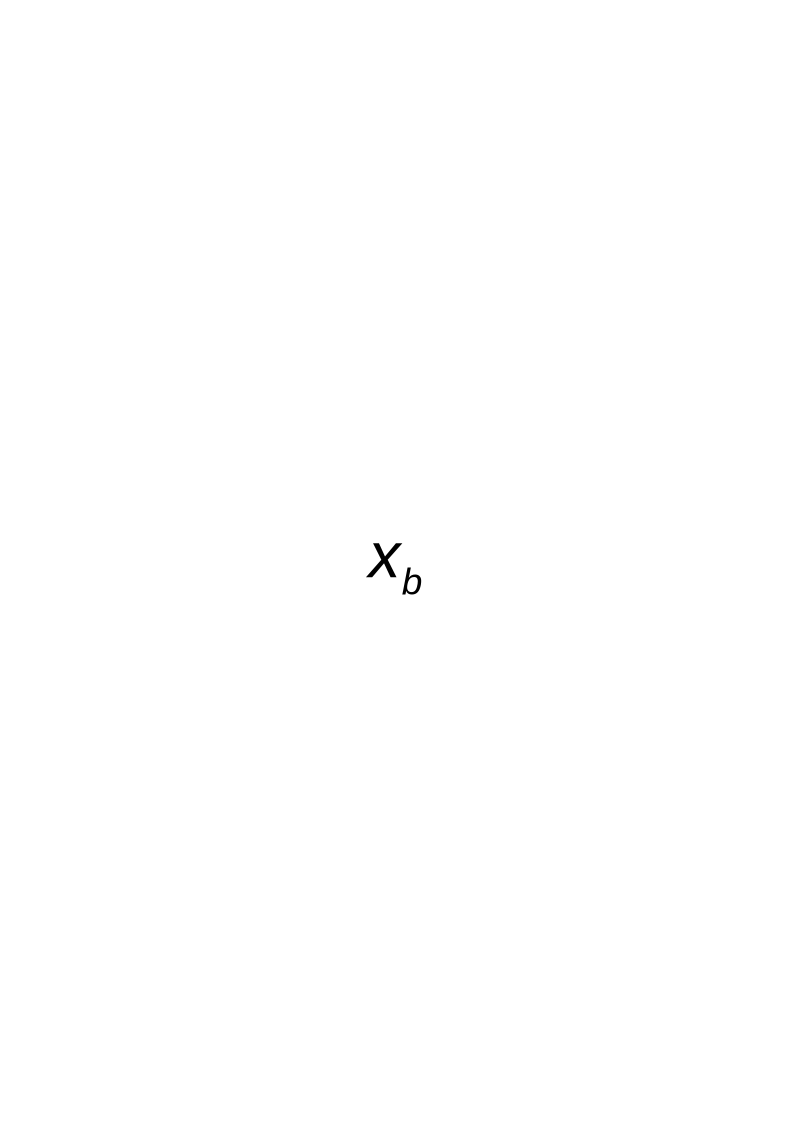
\includegraphics{images/image68.png}

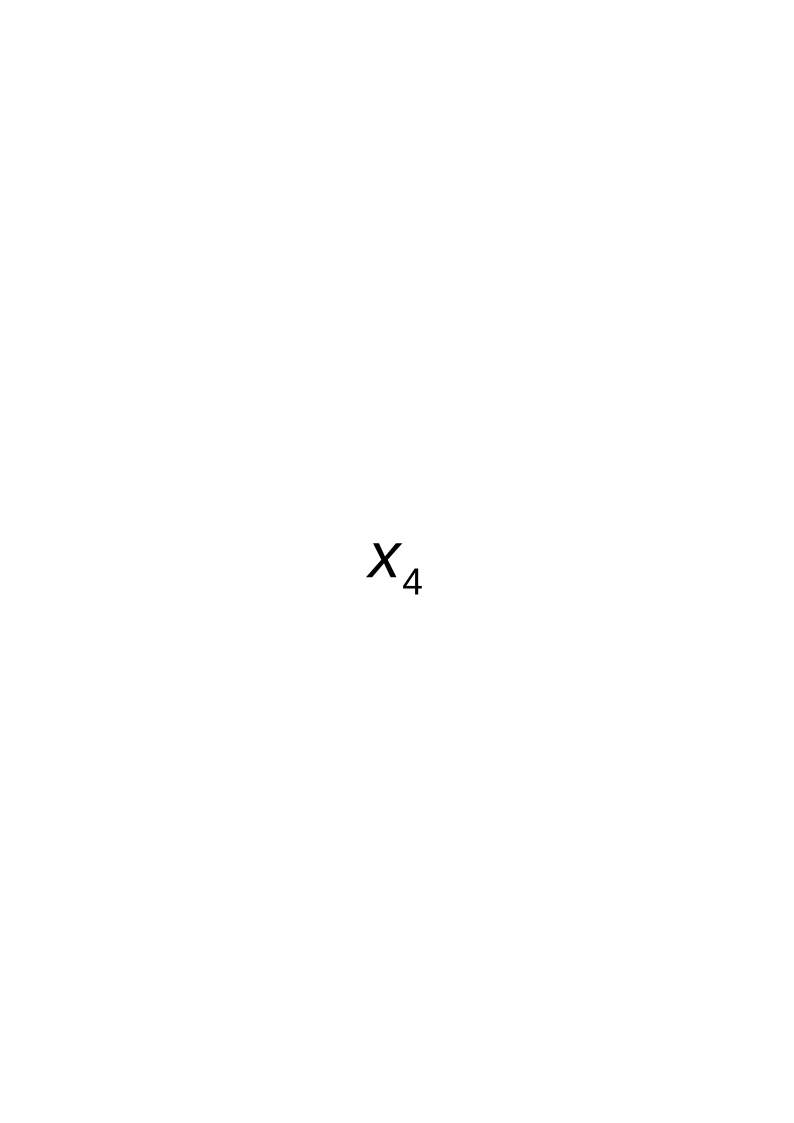
\includegraphics{images/image69.png}


\includegraphics{images/image70.png}


\includegraphics{images/image71.png}

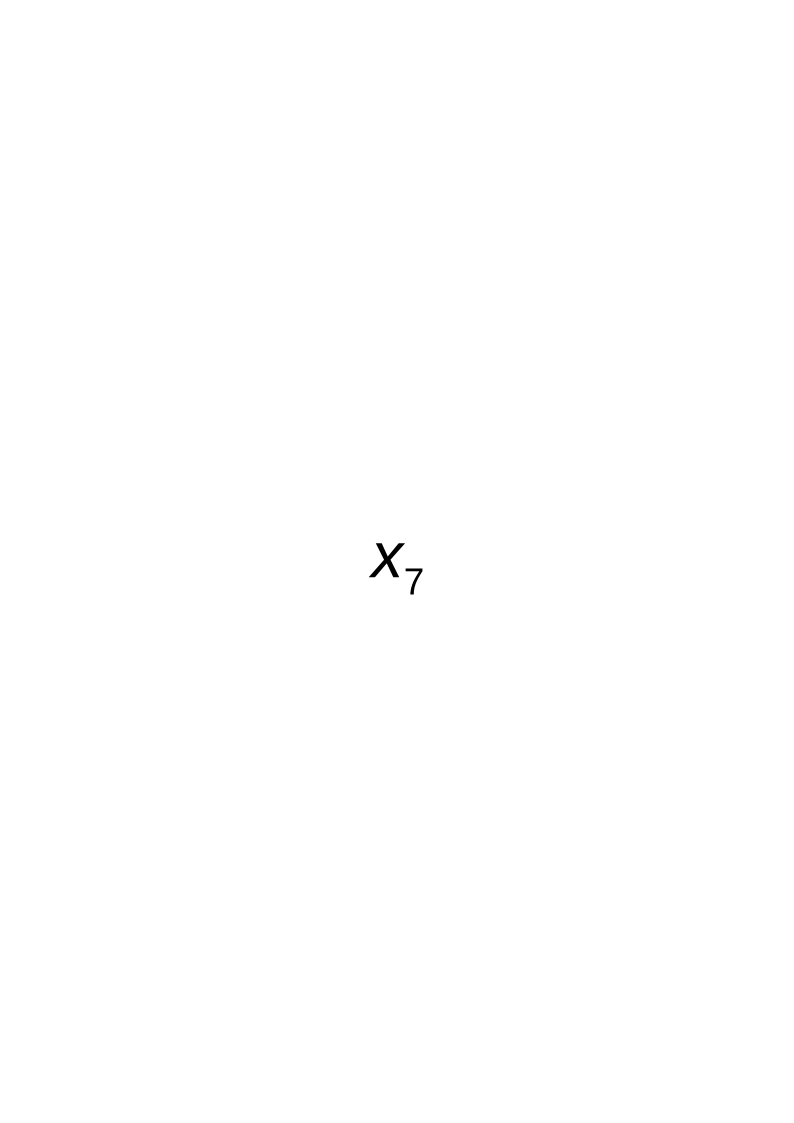
\includegraphics{images/image72.png}

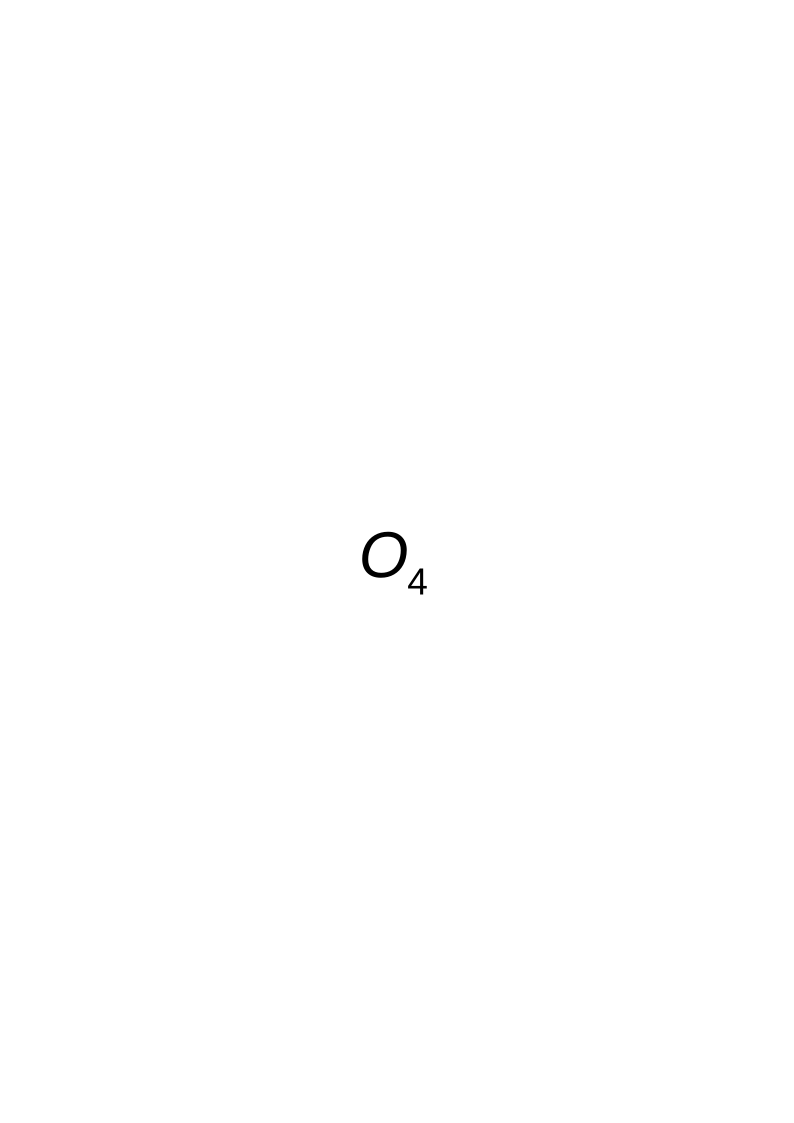
\includegraphics{images/image73.png}

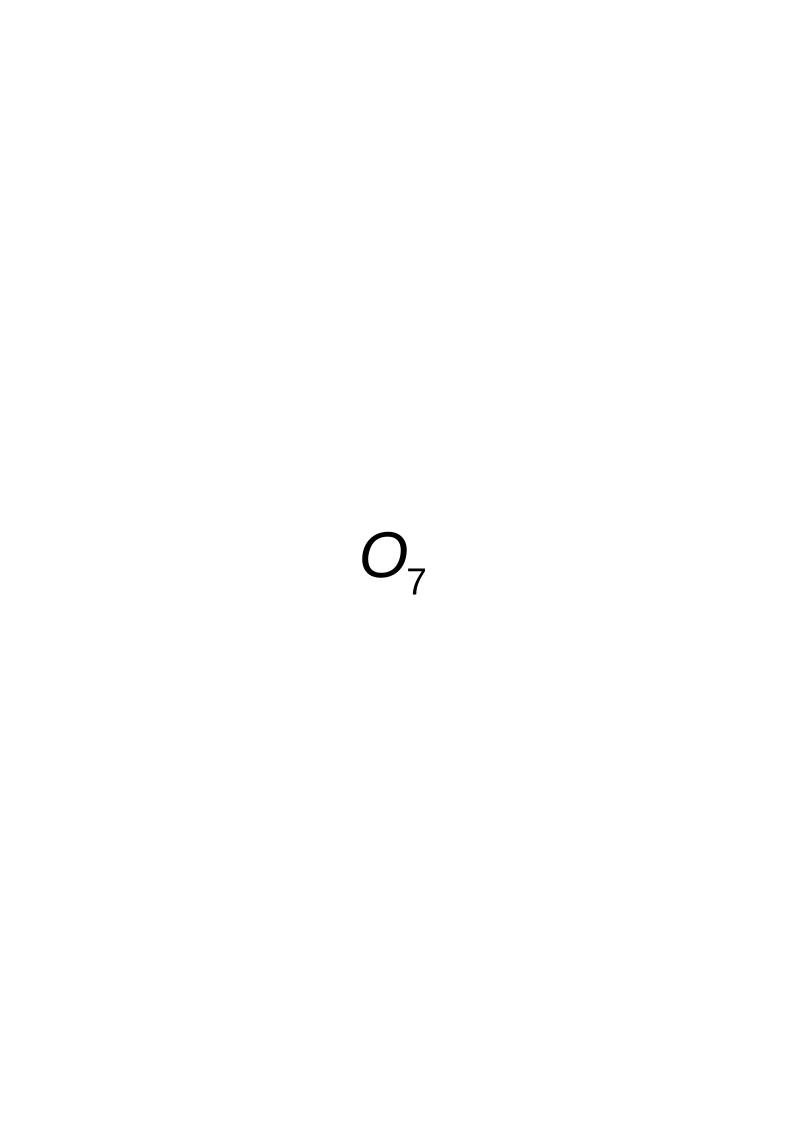
\includegraphics{images/image74.png}

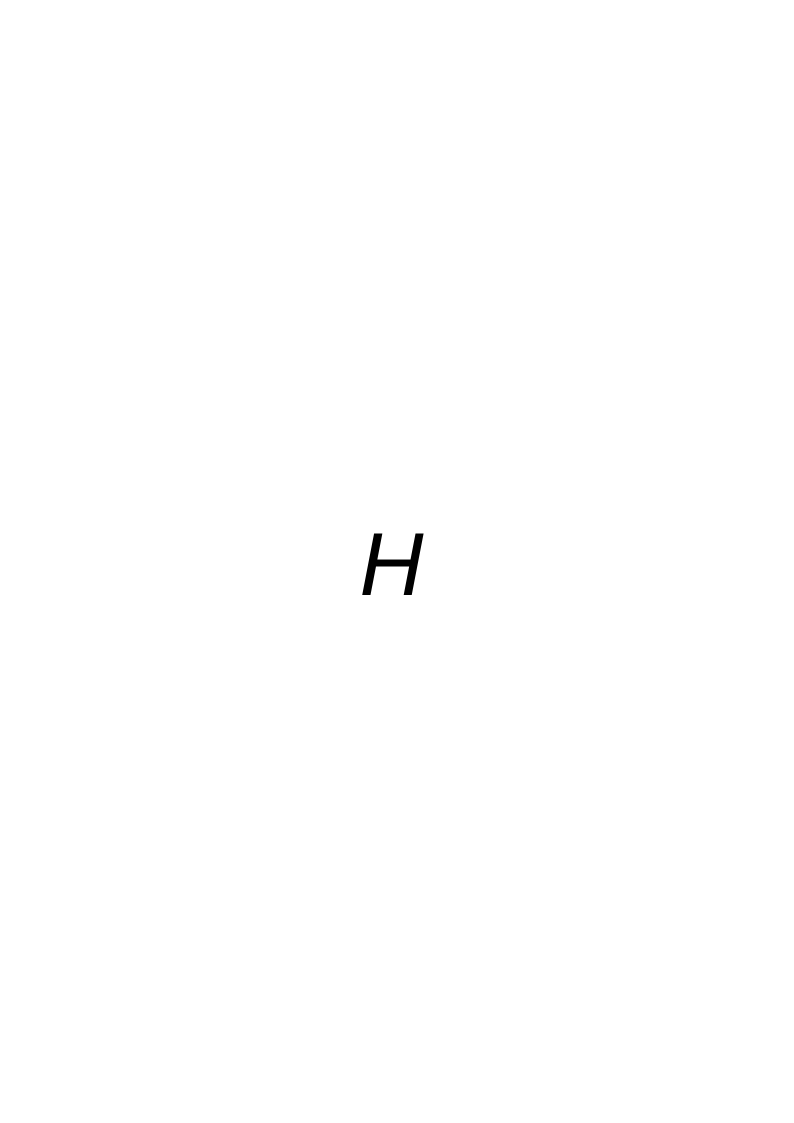
\includegraphics{images/image75.png}

1

1


\includegraphics{images/image76.png}


\includegraphics{images/image77.png}

\textbf{\ul{Modèle cinématique simplifié du dispositif de commande du
PHR.}}

\textbf{ÉCHELLE EPAS}


\includegraphics[width=\linewidth,keepaspectratio]{images/image37.png}
Niveau 1

\emph{(\ul{Source :} Centrale Supélec PSI 2007)}

\textbf{\ul{Objectif de l'étude~:}}

\begin{itemize}
\item
  \textbf{Déterminer} la course minimale du vérin de dressage pour
  pouvoir répondre aux exigences du cahier des charges fonctionnel.

  \begin{enumerate}
  \item
    Mise en situation
  \end{enumerate}
\end{itemize}

Une E.P.A.S. est une Echelle Pivotante Automatique à commande
Séquentielle. Ce système conçu et commercialisé par la société CAMIVA
est monté sur le châssis d'un camion de pompiers et permet de déplacer
une plate-forme pouvant recevoir deux personnes et un brancard le plus
rapidement possible et en toute sécurité.

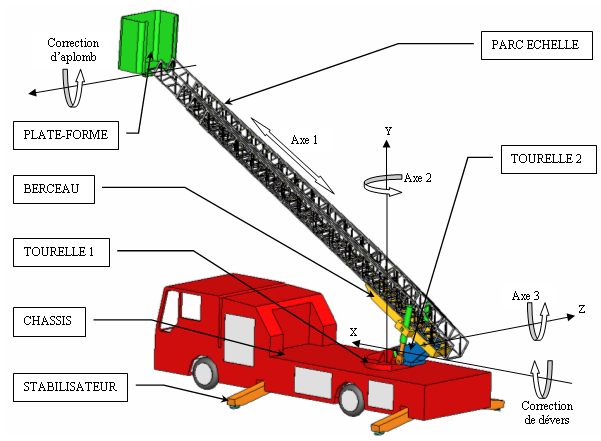
\includegraphics[width=\linewidth,keepaspectratio]{images/image78.png}

Le déplacement de la plate-forme est réalisé suivant trois axes~:

\begin{itemize}
\item
  Le déploiement du parc échelle (axe 1)~: Chaque plan de l'échelle peut
  se translater par rapport aux autres~; seul le quatrième plan
  d'échelle est solidaire du berceau.
\item
  Le pivotement autour de l'axe Y (axe 2)~: La tourelle 1 peut pivoter
  par rapport au châssis autour d'un axe vertical.
\item
  La rotation autour de l'axe Z (axe 3)~: Le berceau peut tourner par
  rapport à la tourelle 2 autour d'un axe horizontal.
\end{itemize}

Pour garantir la sécurité, le système maintient toujours la plate forme
en position horizontale~:

\begin{itemize}
\item
  La correction d'aplomb oriente la plate-forme autour d'un axe
  horizontal parallèle à l'axe Z.
\item
  La correction de devers oriente l'ensemble parc échelle et plate-forme
  autour de l'axe X~: la tourelle 2 s'oriente par rapport à la tourelle
  1 suivant un axe perpendiculaire aux axes 3 et 2.
\end{itemize}

Lors des déplacements suivant les axes 2 et 3, le système «~VARIMAX~» de
commande des actionneurs maintient la vitesse de la plate-forme la plus
constante possible afin de limiter les mouvements de balancier qui
résulteraient d'une commande trop «~brusque~».

Un \ul{système de sécurité} peut, à tout moment, stopper le déplacement
de la plate-forme s'il y a un risque de basculement du camion porteur~:

\begin{itemize}
\item
  Des \ul{capteurs d'efforts} placés sur le parc échelle permettent de
  tenir compte de la charge dans la plate-forme.
\item
  Des \ul{capteurs de position} sur les trois axes permettent de définir
  la position de la plate-forme.
\item
  Des \ul{capteurs inductifs} détectent la position de sortie des
  stabilisateurs.

  \begin{enumerate}
  \item
    Étude géométrique du système de dressage
  \end{enumerate}
\end{itemize}

Pendant la phase de dressage, les tourelles 1 et 2 sont fixes par
rapport au châssis du camion~; seul le berceau pivote autour de l'axe
(A,z) entraînant avec lui le parc échelle et la plate-forme. Ce
mouvement est obtenu grâce aux vérins hydrauliques articulés en B et C
avec la tourelle 2 et le berceau.

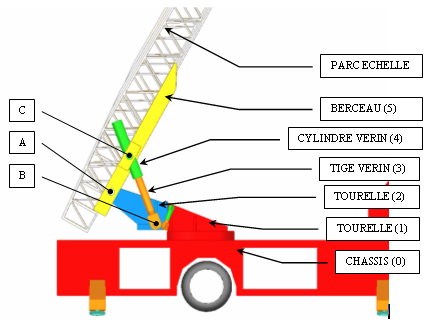
\includegraphics[width=\linewidth,keepaspectratio]{images/image79.png}

On propose le paramétrage suivant~:

Le repère
\(R_{0} = \left( O_{0},{\overrightarrow{x}}_{0},{\overrightarrow{y}}_{0},{\overrightarrow{z}}_{0} \right)\)
est lié au châssis (0).

Le repère
\(R_{5} = \left( A,{\overrightarrow{x}}_{5},{\overrightarrow{y}}_{5},{\overrightarrow{z}}_{0} \right)\)
est lié à l'ensemble \{berceau+parc échelle\} (5)~;

avec \(\overline{O_{0}A} = a\) et
\(\left( {\overrightarrow{x}}_{0};{\overrightarrow{x}}_{5} \right) = \theta\)~;
\(\overline{AC} = c\)~;
\(\overrightarrow{\mathbf{CG}}\mathbf{= L}\mathbf{\cdot}{\overrightarrow{\mathbf{x}}}_{\mathbf{5}}\mathbf{+}\mathbf{h \cdot}{\overrightarrow{\mathbf{y}}}_{\mathbf{5}}\)

Le repère
\(R_{3} = \left( B,{\overrightarrow{x}}_{3},{\overrightarrow{y}}_{3},{\overrightarrow{z}}_{0} \right)\)
est lié la tige du vérin 3~;

avec \(\overline{O_{0}B} = b\)~; \(\overline{BC} = r(t)\) et
\(\left( {\overrightarrow{x}}_{0};{\overrightarrow{x}}_{3} \right) = \beta\)

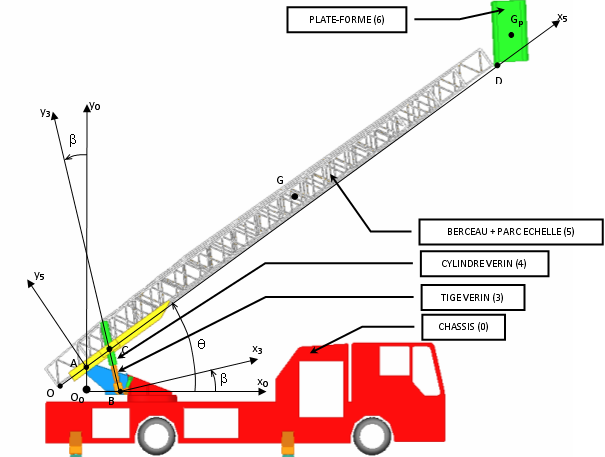
\includegraphics[width=\linewidth,keepaspectratio]{images/image5.png}

\textbf{\ul{Hypothèses~:}}

En raison de la symétrie du système de dressage, nous ne tiendrons
compte que d'un seul vérin hydraulique.

L'action de la pesanteur sur les différents solides sera négligée sauf
pour l'ensemble \{berceau+parc échelle\} de masse M.

Les deux études seront réalisées dans le cas d'un problème plan
\(\mathbf{(}{\overrightarrow{\mathbf{X}}}_{\mathbf{0}}\mathbf{,}{\overrightarrow{\mathbf{Y}}}_{\mathbf{0}}\mathbf{)}\)

\includesvg[width=5.48822in,height=3.36458in]{images/image7.svg}

\begin{enumerate}
\def\labelenumi{\arabic{enumi}.}
\item
  ~\textbf{Déterminer} la loi entrée/sortie du système de dressage.
\item
  \textbf{~En déduire} la course minimale du vérin de dressage pour
  pouvoir passer de la position basse de l'échelle (θ=10°) à la position
  haute (θ=50°).
\end{enumerate}

\emph{On prendra c=2,6m~; a=2m, b=3m}


\includegraphics[width=\linewidth,keepaspectratio]{images/image80.jpeg}\textbf{STABILISATEUR
CARDIAQUE ACTIF}


\includegraphics[width=\linewidth,keepaspectratio]{images/image37.png}
Niveau 3

\emph{(\ul{Source :} Centrale Supélec TSI 2012)}

\textbf{\ul{Objectif de l'étude~:}}

\begin{itemize}
\item
  \textbf{Déterminer} la course de l'actionneur piézoélectrique pour
  couvrir l'espace de travail.

  \begin{enumerate}
  \item
    Mise en situation
  \end{enumerate}
\end{itemize}

Les pathologies cardiaques et particulièrement les sténoses
(rétrécissements des artères) alimentant le muscle cardiaque sont en
constantes augmentations. La chirurgie à cœur battant se substitue
progressivement à celle courante constituée par un arrêt du cœur et par
la mise en place d'une circulation extracorporelle. L'un des avantages
essentiels de cette chirurgie à cœur battant est de limiter les
complications induites par l'intervention.

Cette technique opératoire se différencie du pontage classique par la
conservation du battement cardiaque durant l'intervention~; la
principale difficulté réside alors dans la nécessité d'immobiliser la
partie du cœur à opérer.

Pour intervenir précisément sur la zone concernée, il est nécessaire de
faire appel à un stabilisateur mécanique qui immobilise cette «~zone
cible~».

Actuellement, les stabilisateurs mécaniques laissent subsister pour
cette zone un déplacement résiduel (de l'ordre du mm) alors que la
précision requise est plutôt de 0,1 mm. De plus, cette précision est
insuffisante en vue d'une utilisation endoscopique, technique
d'intervention dont le développement va croissant.

La solution proposée pour remédier à ces insuffisances est celle
constituée par un \emph{stabilisateur cardiaque actif},
c\textquotesingle est-à-dire commandé en position. Dans le cas de notre
étude, il s'agit du système «~Cardiolock1~» développé principalement au
laboratoire du LSIIT de l'Université de Strasbourg.

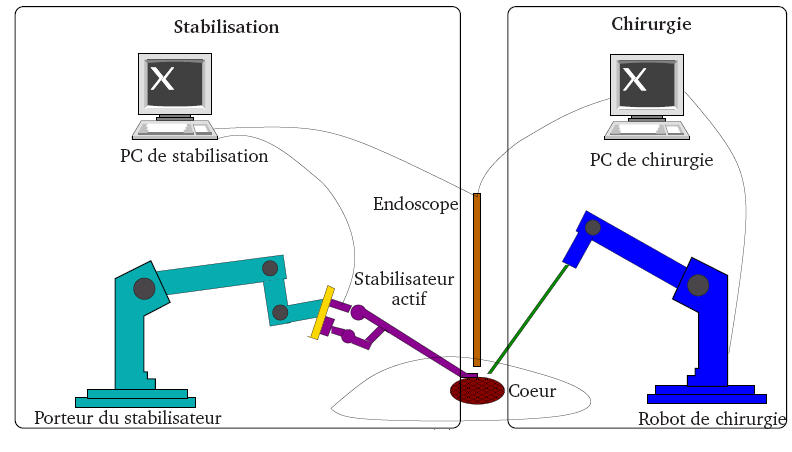
\includegraphics[width=\linewidth,keepaspectratio]{images/image81.jpeg}

\textbf{Figure 1}. Contexte d'utilisation du Cardiolock1

\textbf{Présentation du Cardiolock1}

Les amplitudes peu élevées des mouvements considérés et la recherche de
liaisons sans jeu, justifient l'emploi d'un mécanisme constitué de
«~liaisons pivots élastiques~»~: celles-ci sont obtenues en combinant
l'élasticité du matériau et la géométrie des pièces (amincissement
résultant d'un enlèvement de matière localisé) de façon à favoriser une
déformation locale de la pièce qui permet d'obtenir le comportement
d'une liaison pivot sans jeu.

\textbf{Figure 2}. Représentation du cardiolock1

La tige est stérilisable par autoclave, quant au système d'actionnement,
il peut être protégé par un sac stérile.

Dans toute l'étude, on retiendra les hypothèses suivantes~:

\begin{itemize}
\item
  L'étude envisagée est faite dans le cadre d'une modélisation plane~;
  le repère
  \(\left\{ O,{{\overrightarrow{x}}_{0},\overrightarrow{y}}_{0},{\overrightarrow{z}}_{0}\  \right\}\)
  est lié au bâti \textbf{0} et est supposé galiléen~; le déplacement
  résiduel à rattraper est supposé positif sur
  \({\overrightarrow{y}}_{0}\ \).
\item
  Les déplacements envisagés sont de petits déplacements, par suite, on
  confondra dans toute la suite, au voisinage de 0, le sinus de l'angle
  avec sa mesure en radian ou encore le cosinus avec 1.
\item
  Les liaisons pivots élastiques, sans jeu (dans la suite du texte,
  notée en abrégé: pivot*), sont obtenues par enlèvement de matière et
  se comportent comme une liaison pivot parfaite à laquelle s'ajoute de
  manière indissociable une raideur de torsion générant un couple de
  rappel porté par l'axe de la liaison.
\end{itemize}

Un modèle cinématique du stabilisateur est défini par les figures 3, 4
et 5.


\includegraphics[width=\linewidth,keepaspectratio]{images/image83.png}

\textbf{Figure 3}. Graphe des liaisons


\includegraphics[width=\linewidth,keepaspectratio]{images/image84.png}

\textbf{Figure 4}. Paramétrage des rotations

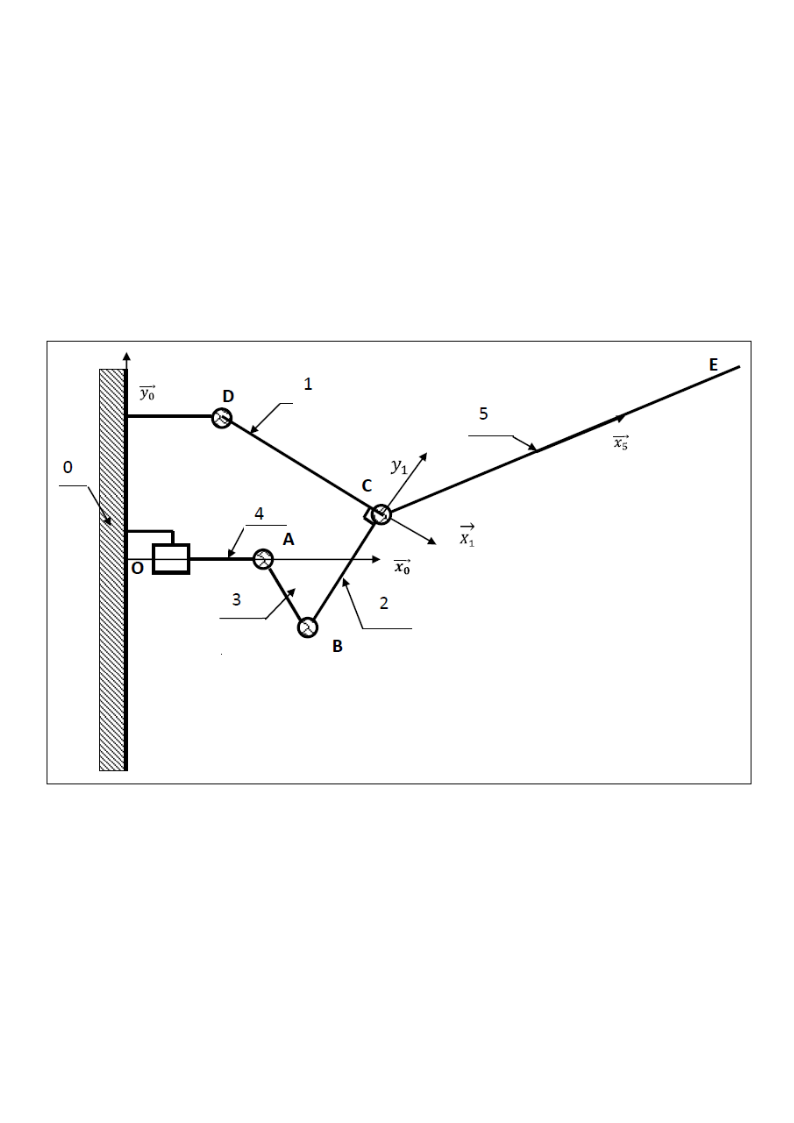
\includegraphics[width=\linewidth,keepaspectratio]{images/image85.png}

\textbf{Figure 5}. Schéma cinématique du cardiolock1

\emph{\textbf{Evaluation de l'espace de travail}}

On envisage l'évolution quasi-statique du système à partir de la
configuration dite de repos (pour laquelle les paramètres α, β,
\(\gamma\) sont égaux à zéro) avec l'objectif de déterminer l'espace de
travail.

\textbf{I.A.1} \emph{\textbf{Détermination du déplacement extremum du
point E dû à l'actionneur piézoélectrique}}

On calcule les expressions de \(\lambda\) et \(\gamma\) en fonction de α
et des paramètres géométriques afin d'en déduire les déplacements du
point C puis du point E.

\begin{enumerate}
\def\labelenumi{\arabic{enumi}.}
\item
  Ecrire la fermeture géométrique de la chaîne fermée
  \textbf{0}-\textbf{1}-\textbf{2}-\textbf{3}-\textbf{4}-\textbf{0} et
  en déduire le système d'équations liant λ, α, \(\gamma\) aux
  paramètres géométriques \(\ a,\ \ L1,\ \ L3,\ \ d1\)\textsubscript{.}
  Linéariser ce système et exprimer ensuite \(\lambda\) et \(\gamma\) en
  fonction de α
\item
  Exprimer la valeur λ\textsubscript{0} prise par λ dans la
  configuration de repos, en déduire l'expression du déplacement
  \(x_{A} = \lambda - \lambda_{0}\) en fonction de α et \(d_{1}\).
  Donner le signe de \(x_{A}\) permettant le rattrapage d'un déplacement
  positif selon \({\overrightarrow{y}}_{0}\ \)de l'extrémité E de la
  tige \textbf{5}.
\end{enumerate}

On note \(x_{Aex}\)le déplacement extrémum égale à \(- 130\mu m\),
déterminer les expressions de \(\gamma\) et α dans ce cas, elles seront
notées respectivement \(\alpha_{ex}\) et \(\gamma_{ex}\). Faire les
applications numériques.

\begin{enumerate}
\def\labelenumi{\arabic{enumi}.}
\setcounter{enumi}{2}
\item
  Exprimer en fonction de L\textsubscript{1} et α le déplacement
  \(y_{C}\) du point C (dans le repère
  \(\left\{ O,{{\overrightarrow{x}}_{0},\overrightarrow{y}}_{0},{\overrightarrow{z}}_{0}\  \right\}\).
  Faire l'application numérique pour \(\alpha = \alpha_{ex}\), on notera
  \(y_{Cex}\) cette valeur numérique. En déduire le déplacement extremum
  du point E, noté \(y_{Eex}\).
\end{enumerate}


\includegraphics[width=\linewidth,keepaspectratio]{images/image86.png}\textbf{COMPACTEUR
CATERPILAR}


\includegraphics[width=\linewidth,keepaspectratio]{images/image37.png}
Niveau 2

\emph{(\ul{Source :} Jérôme Letard, Concours Centrale Supélec 2004)}

\textbf{\ul{Objectif de l'étude~:}}

\begin{itemize}
\item
  \textbf{Déterminer} la course du vérin hydraulique permettant
  d'obtenir le débattement angulaire souhaité par le cahier des charges.

  \begin{enumerate}
  \item
    Mise en situation
  \end{enumerate}
\end{itemize}


\includegraphics{images/image87.png}

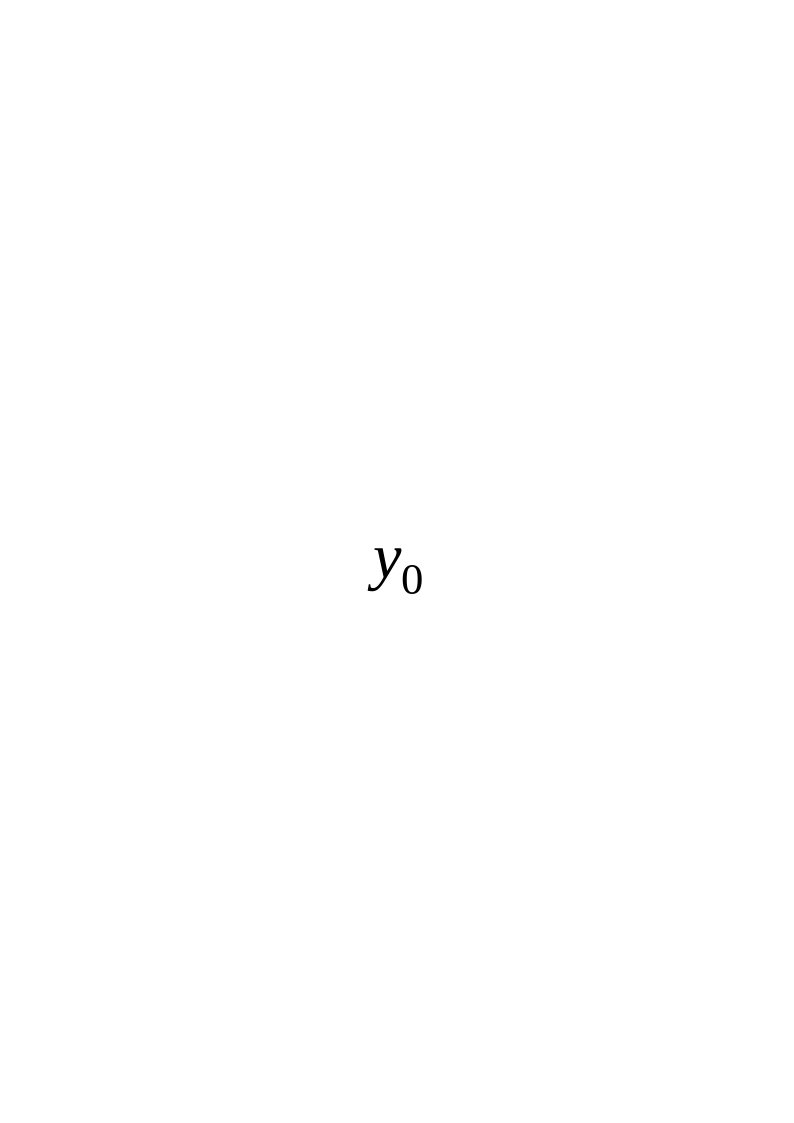
\includegraphics{images/image88.png}


\includegraphics{images/image89.png}


\includegraphics[width=\linewidth,keepaspectratio]{images/image90.png}Le
compacteur étudié (Caterpillar,modèle CB-214D ) est présenté sur les
figures ci dessous avec ses caractéristiques externes principales.

Ce compacteur vibrant est destiné aux petits travaux de compactage. Pour
ce type d'engin, le compactage résulte plus des chocs à fréquence élevée
qu'exerce chaque cylindre sur le sol plutôt que de la masse du
compacteur.

Moteur de cylindre arrière

Support de cylindre arrière

Cylindre arrière

cylindre avant

½ bâti avant

½ bâti arrière

Moteur d'avancement avant

Support de cylindre avant


\includegraphics[width=\linewidth,keepaspectratio]{images/image93.png}


\includegraphics{images/image89.png}

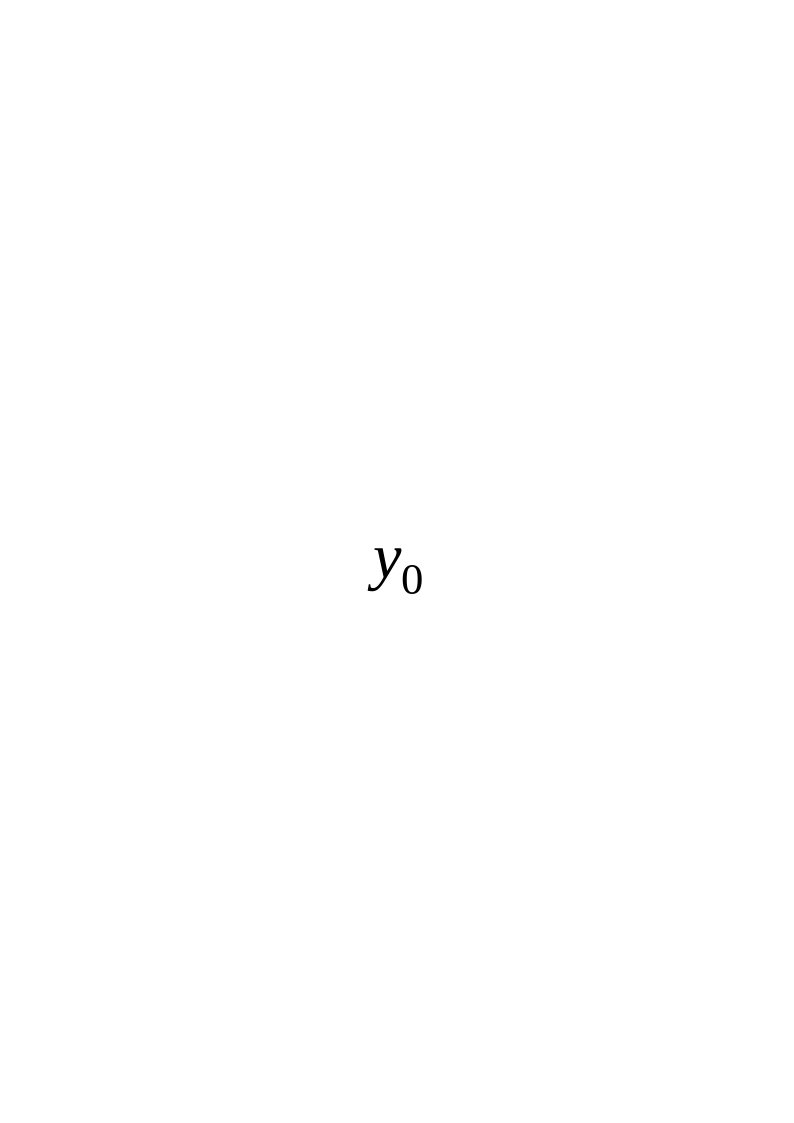
\includegraphics{images/image88.png}

\emph{B}

\emph{I}

En fonctionnement normal le compacteur réalise tout type de trajectoire.

Les \textbf{solutions constructives} qui ont été choisies lors de sa
conception doivent donc permettre de répondre à la \textbf{fonction
\emph{\ul{FC3}}}\emph{\ul{~: \textbf{changer de direction le
véhicule.}}}

Le choix effectué ici est une articulation entre la partie avant et la
partie arrière commandée par un vérin hydraulique. \emph{(Voir schéma
cinématique du système d'orientation des cylindres)}

Il s'agit de traiter du problème d'orientation des deux demi-bâtis (et
donc des cylindres) lorsque le compacteur se déplace en courbe.

\textbf{L'angle Ø entre le cylindre avant et arrière doit être compris
entre -32° et + 32°} (courbe vers la droite ou vers la gauche).

\begin{enumerate}
\setcounter{enumi}{1}
\item
  Modélisation du mécanisme
\end{enumerate}

\begin{enumerate}
\def\labelenumi{\arabic{enumi}.}
\item
  \textbf{Déterminer} les classes d'équivalence.
\item
  \textbf{Établir} le graphe des liaisons.

  \begin{enumerate}
  \item
    Détermination de la course du vérin hydraulique
  \end{enumerate}
\item
  \textbf{Paramétrer} le système.
\item
  \textbf{Déterminer} la loi entrée sortie du mécanisme\emph{.}
\item
  \textbf{En déduire} la course minimale c du vérin afin de répondre au
  critère du cahier des charges\\
  (-32°\textless Ø\textless+32°).
\end{enumerate}

\textbf{\ul{Schéma cinématique fonctionnel du système d'orientation des
cylindres de compactage}}

\textbf{BARRIERE SINUSMATIC}


\includegraphics[width=\linewidth,keepaspectratio]{images/image37.png}
Niveau 3

\begin{enumerate}
\item
  Train d'engrenages simple
\end{enumerate}

Le système "SINUSMATIC" (conçu par la société ELLIPSE INDUSTRIE) est un
système automatisé permettant la fermeture et l'ouverture d'une barrière
de type péage d'autoroute, parking, etc...

Moteur à courant continu

Réducteur à engrenages

\emph{\textbf{SINUSMATIC}}

Barrière de parking


\includegraphics[width=\linewidth,keepaspectratio]{images/image97.png}Sa
particularité résulte de la cinématique de son renvoi
d\textquotesingle angle \textbf{irréversible} qui transforme le
mouvement de rotation continu du plateau \textbf{7} lié à l'axe du
motoréducteur en mouvement de rotation alternatif (1/4 de tour) de la
barrière liée à l'arbre de sortie \textbf{2} du mécanisme. A chaque
demi-tour du plateau \textbf{7} correspond une position haute ou basse
de la barrière.

Ce système Sinusmatic est représenté sous la forme des schémas
cinématiques ci-dessous~:


\includegraphics[width=\linewidth,keepaspectratio]{images/image98.png}
\includegraphics[width=\linewidth,keepaspectratio]{images/image100.png}

\emph{\ul{Constituants et paramétrage~:}}

\begin{itemize}
\item
  \(R_{1}(A,\overrightarrow{x},\overrightarrow{y},\overrightarrow{z})\)
  est associé au bâti \textbf{1} considéré comme fixe.
\item
  \(R_{7}(A,\overrightarrow{x_{7}},\overrightarrow{y_{7}},\overrightarrow{z})\)
  est associé au plateau \textbf{7}, tel que
  \(\alpha = (\overrightarrow{y},\overrightarrow{y_{7}})\).
\item
  \(R_{3}(C,\overrightarrow{x_{7}},\overrightarrow{y_{3}},\overrightarrow{z_{3}})\)
  est associé au croisillon \textbf{3}, tel que
  \(\gamma = (\overrightarrow{y_{7}},\overrightarrow{y_{3}}) = Cte = 45{^\circ}\).
\item
  \(R_{2}(C,\overrightarrow{x_{2}},\overrightarrow{y},\overrightarrow{z_{2}})\)
  est associé à l'arbre \textbf{2}, tel que
  \(\beta = (\overrightarrow{x},\overrightarrow{x_{2}})\).
\end{itemize}


\includegraphics[width=\linewidth,keepaspectratio]{images/image101.png}

\emph{\textbf{\ul{Objectif~:}} Vérifier le critère de la fonction FC2.}

\textbf{Q1.} Donner le paramètre d'entrée et le paramètre de sortie du
système.

\textbf{Q2.} Dessiner le graphe des liaisons de ce système.

\textbf{Q5}. Représenter les figures planes de changement de base
relatives aux angles \protect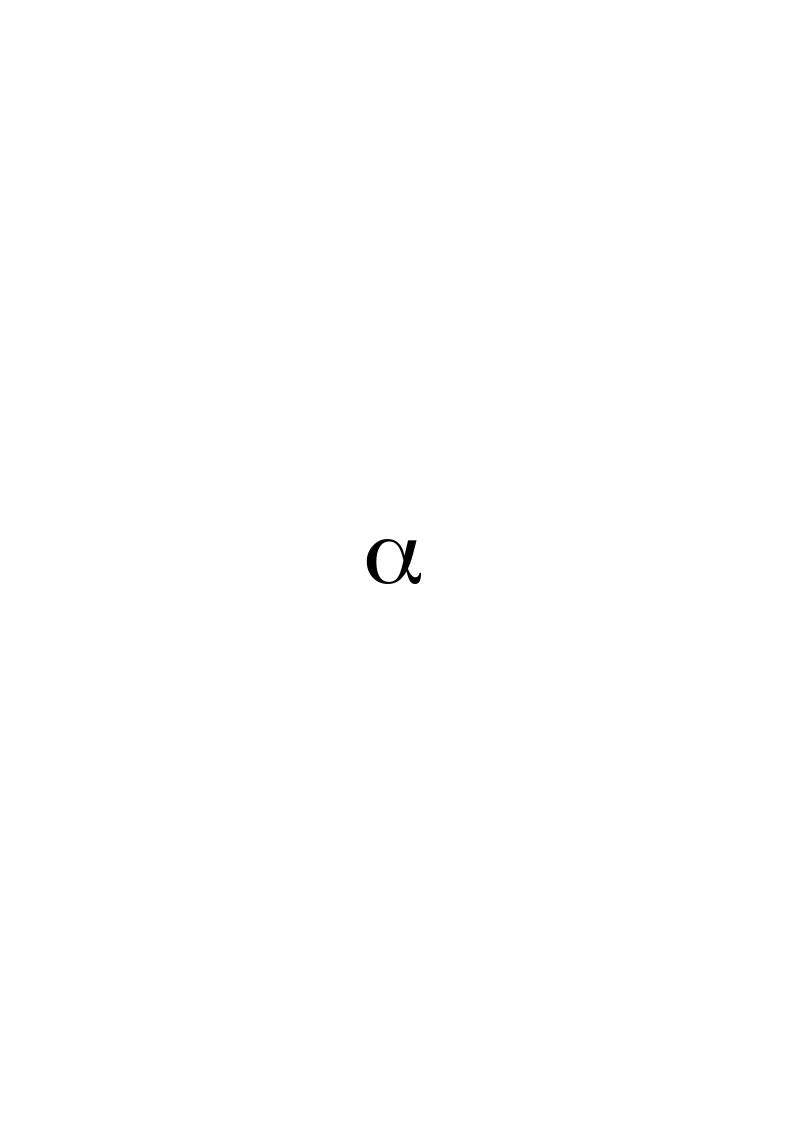
\includegraphics{images/image102.png},
\protect
\includegraphics{images/image103.png}et~\protect
\includegraphics{images/image104.png}.

\textbf{Q6}. Déterminer à partir de la particularité géométrique
\(\overrightarrow{y_{3}}\bot\overrightarrow{x_{2}}\), la loi
entrée-sortie en position du système.

\textbf{Q7.} Conclure quant au respect du critère de la fonction FC2.

\textbf{MECANISME OSCILLANT}


\includegraphics[width=\linewidth,keepaspectratio]{images/image37.png}
Niveau 1


\includegraphics[width=\linewidth,keepaspectratio]{images/image105.png}

\textbf{MECANISME A CAME}


\includegraphics[width=\linewidth,keepaspectratio]{images/image37.png}
Niveau 1

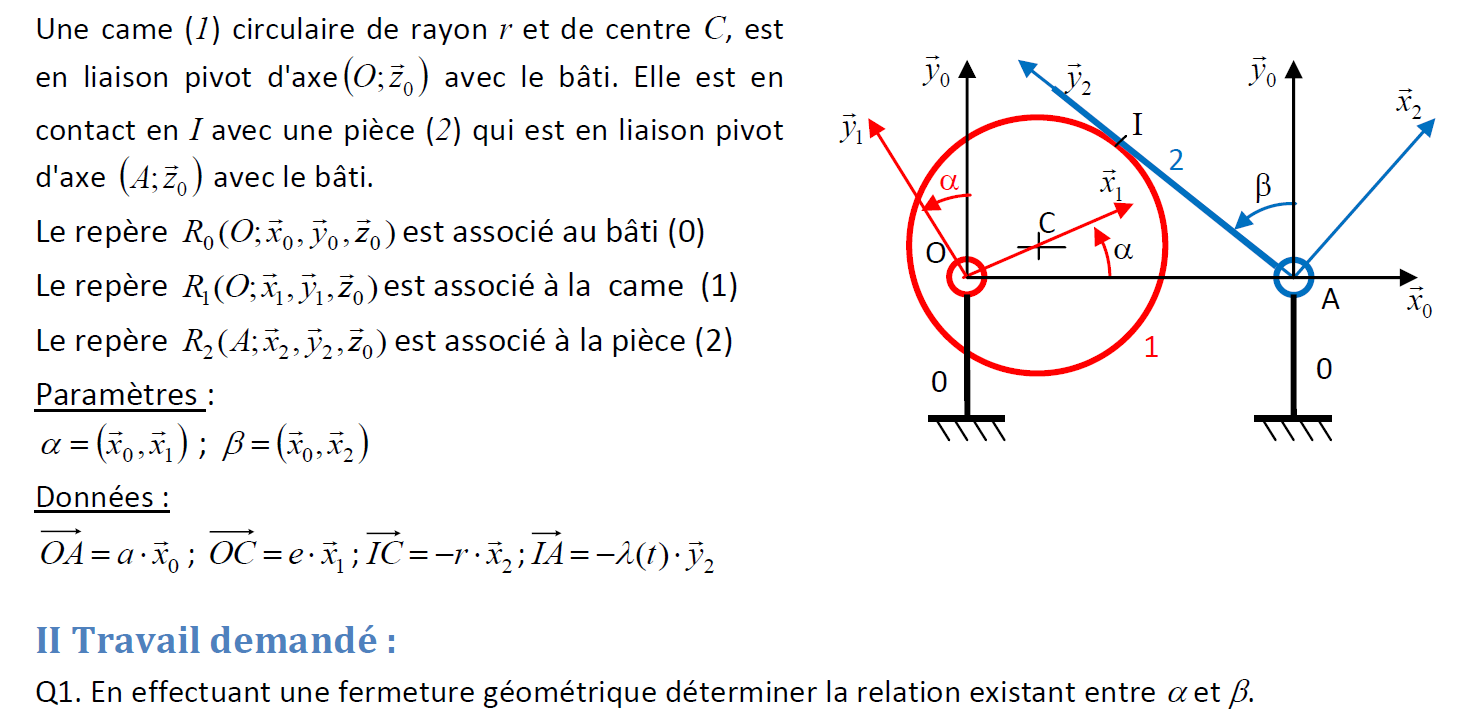
\includegraphics[width=\linewidth,keepaspectratio]{images/image106.png}

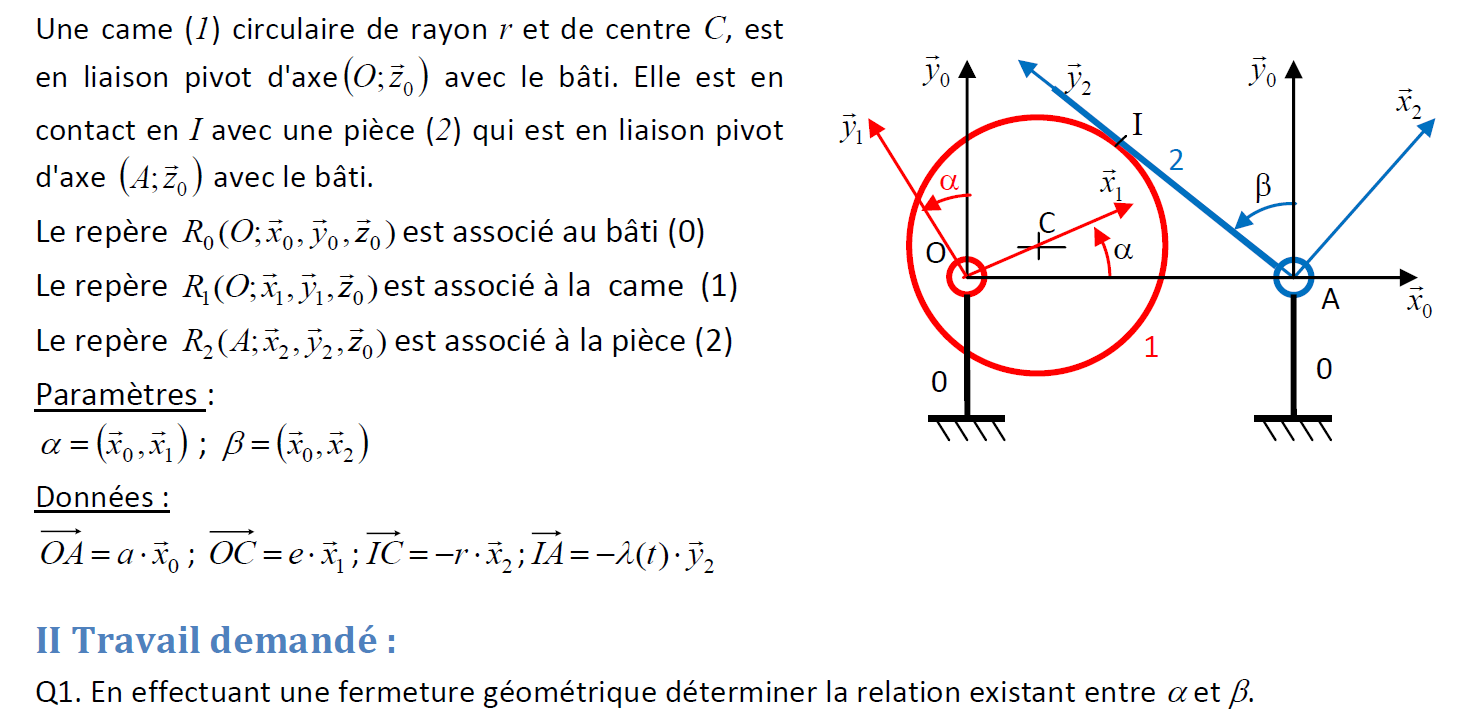
\includegraphics[width=\linewidth,keepaspectratio]{images/image106.png}

\textbf{BRAS DE ROBOT}


\includegraphics[width=\linewidth,keepaspectratio]{images/image37.png}
Niveau 1

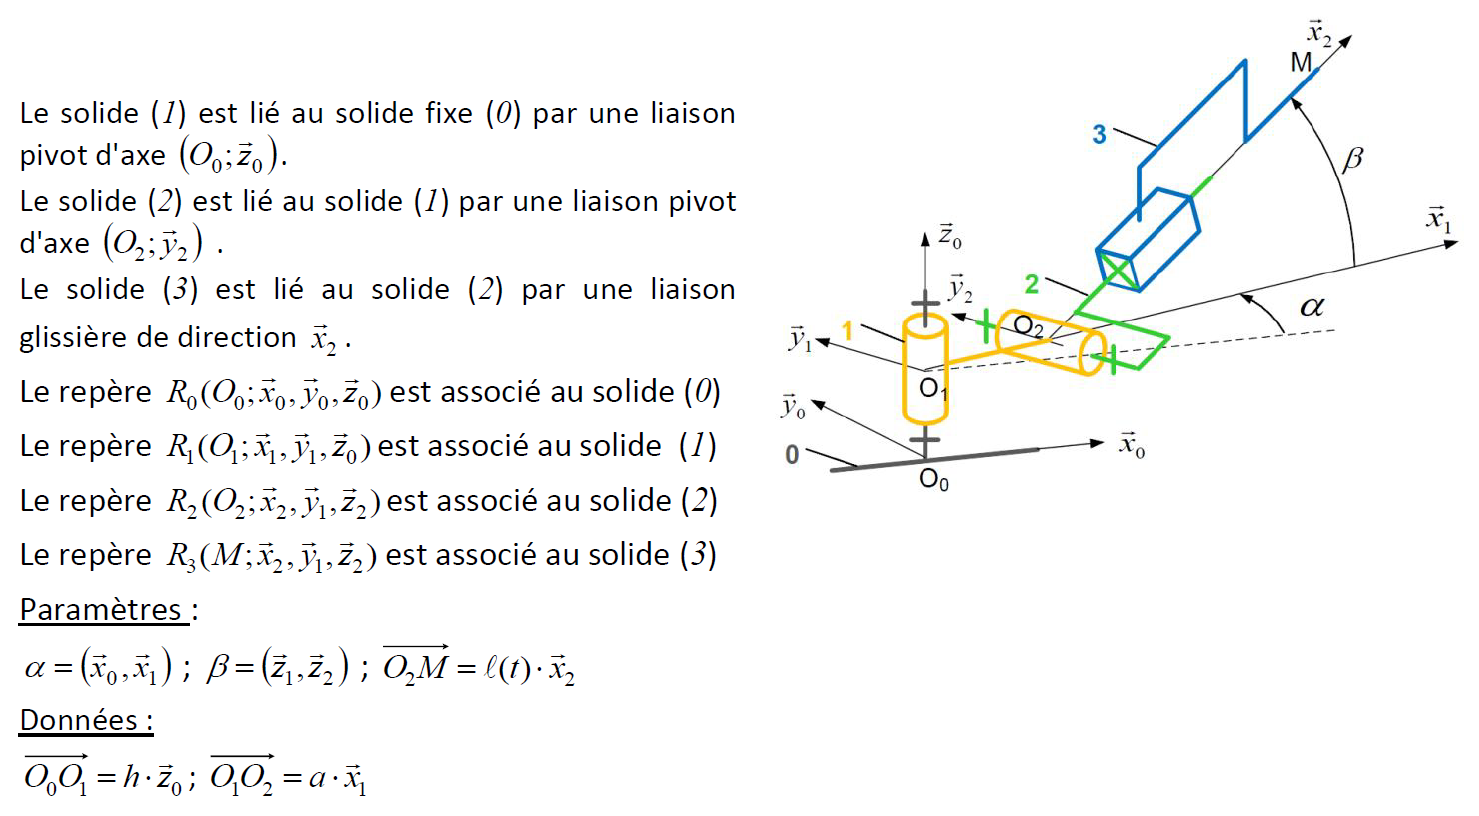
\includegraphics[width=\linewidth,keepaspectratio]{images/image107.png}


\includegraphics[width=\linewidth,keepaspectratio]{images/image108.png}

\textbf{POMPE OSCILLANTE}


\includegraphics[width=\linewidth,keepaspectratio]{images/image37.png}
Niveau 2


\includegraphics[width=\linewidth,keepaspectratio]{images/image109.png}

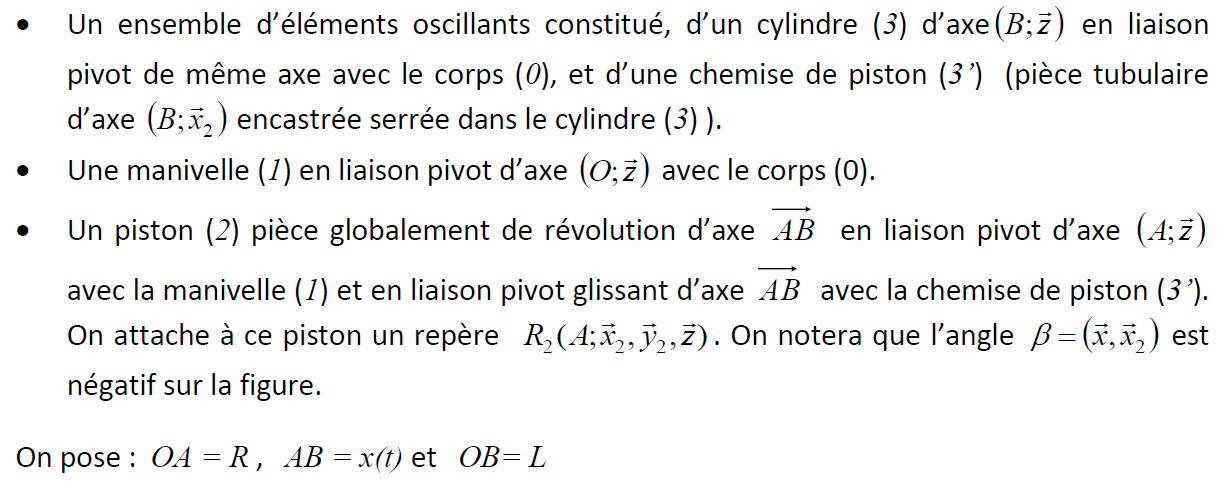
\includegraphics[width=\linewidth,keepaspectratio]{images/image110.png}


\includegraphics[width=\linewidth,keepaspectratio]{images/image111.png}

\textbf{BANC D'EPREUVE HYDRAULIQUE}


\includegraphics[width=\linewidth,keepaspectratio]{images/image37.png}
Niveau 2


\includegraphics[width=\linewidth,keepaspectratio]{images/image112.png}


\includegraphics[width=\linewidth,keepaspectratio]{images/image113.png}


\includegraphics[width=\linewidth,keepaspectratio]{images/image114.png}


\includegraphics[width=\linewidth,keepaspectratio]{images/image115.png}\textbf{SYSTEME
D'AGITATION POUR LES CELLULES PANCREATIQUES}


\includegraphics[width=\linewidth,keepaspectratio]{images/image37.png}
Niveau 3

(\ul{Source : CCP PSI} 2010)


\includegraphics[width=\linewidth,keepaspectratio]{images/image116.png}Dans
le cadre d'expérimentations pour soigner les malades du diabète, une
équipe de chercheurs travaille sur une technique de greffe de cellules
du pancréas.

Ces cellules sont obtenues à partir d'un pancréas issu d'un don
d'organes.

Elles sont isolées du pancréas puis purifiées. Ces dernières,
responsables de la sécrétion d'insuline, sont, après un maintien en
culture (24 à 48 heures) greffées à un patient diabétique.

Afin d'isoler les cellules, on place des fragments de pancréas au sein
d'une petite enceinte thermostatée (photo 1). On a préalablement injecté
un mélange d'enzymes à l'intérieur du pancréas. Une fois placés dans
l'enceinte, les fragments de pancréas vont «baigner» dans cette enzyme,
ce qui va enclencher un phénomène de digestion. Tout au long de la
manipulation, la solution va circuler, dans un circuit fermé constitué
de l'enceinte, de tuyaux et d'une pompe. Pour faciliter l'action de
l'enzyme, l'opération se fait sous agitation permanente.

La digestion est aussi facilitée par le mouvement de billes en acier au
sein de l'enceinte. L'agitation dure 1h30 à 2h30 et doit permettre la
libération et la récolte des cellules du pancréas.

Nous allons dans la suite étudier le système d'agitation et de chauffage
de l'enceinte thermostatée (photo 1 et plan A4).

\paragraph*{Description de l'agitateur et du système de
chauffage~:}\label{description-de-lagitateur-et-du-systuxe8me-de-chauffage}
\addcontentsline{toc}{paragraph}{Description de l'agitateur et du
système de chauffage~:}

\begin{itemize}
\item
  Le système doit permettre l'agitation de l'enceinte par des mouvements
  continus alternatifs de bas en haut (100 mm) et par des mouvements de
  rotation alternée (+/- 45°) (ces derniers mouvements n'étant réalisés
  qu'un nombre réduit de fois durant la manipulation).
\item
  L'agitateur est suffisamment compact pour pouvoir s'intégrer dans une
  hotte permettant sa stérilisation. Sa manipulation par le chercheur
  doit être facile.
\item
  Le dispositif est constitué de matériaux et de composants respectant
  l'atmosphère de la salle blanche.
\item
  L'enceinte est maintenue à une température constante de 37°C pendant
  la digestion. La température de 37°C est produite par un collier
  chauffant disposé autour de l'enceinte. Ce collier chauffe la solution
  qui circule dans le circuit fermé.
\item
  L'enceinte thermostatée s'adapte sur le système d'agitation.
  L'enceinte est d'un encombrement minimum pour pouvoir s'adapter au
  sein de la hotte à flux laminaire, sachant que d'autres équipements
  tels que les rampes de robinets, la tuyauterie, la pompe
  péristaltique, le système de chauffage doivent également être présents
  à l'intérieur de la hotte. Cette hotte permet de réaliser la
  stérilisation de tous les appareillages.
\end{itemize}

Le système est composé de deux chaînes cinématiques indépendantes (cf.
plan de l'agitateur A4)~:

\begin{itemize}
\item
  chaîne n°1 (principale) constituée d'une machine à courant continu
  \textbf{M\textsubscript{1}}, d'un excentrique \textbf{1}, d'une bielle
  \textbf{2} et du bras \textbf{3} sur lequel est montée la seconde
  chaîne cinématique~;
\item
  chaîne n°2 (secondaire) constituée d'un moto-réducteur électrique
  \textbf{M\textsubscript{2 }}solidaire du bras 3, d'un excentrique,
  d'une bielle et de l'ensemble \{pince, enceinte\}.
\end{itemize}

Le schéma cinématique partiel de la chaine n°1 est donné ci-dessous~:


\includegraphics[width=\linewidth,keepaspectratio]{images/image117.png}

\textbf{\ul{Objectif~N°1:} Déterminer les équations permettant d'obtenir
la loi entrée/sortie~en vitesse et en position.}

\ul{Données~:} \(O_{1}O_{2} = e\)~; \(O_{2}B = b\)~; \(O_{3}B = L\)~;
\(\overrightarrow{O_{3}O_{1}} = c\overrightarrow{x} - d\overrightarrow{y}\)~;\(\overrightarrow{O_{3}A} = q{\overrightarrow{x}}_{3}\)~;
q=400mm

\(\theta_{1} = (\overrightarrow{x},{\overrightarrow{x}}_{1})\)~;
\(\theta_{2} = ({\overrightarrow{x}}_{1},{\overrightarrow{x}}_{2})\)~;
\(\theta_{3} = (\overrightarrow{x},{\overrightarrow{x}}_{3})\)

la base directe R
\includegraphics{images/image118.png} est associée au
bâti~\textbf{0};

la base directe R\textsubscript{1}
\includegraphics{images/image119.png}
est associée à l'excentrique \textbf{1}~;

la base directe
R\textsubscript{2}\(({\overrightarrow{x}}_{2},{\overrightarrow{y}}_{2},\overrightarrow{z})\)
est associée à la bielle \textbf{2}~;

la base directe
R\textsubscript{3}\(({\overrightarrow{x}}_{3},{\overrightarrow{y}}_{3},\overrightarrow{z})\)
est associée au bras \textbf{3}~;

\begin{enumerate}
\def\labelenumi{\arabic{enumi}.}
\item
  A l'aide d'une fermeture géométrique, écrire le système de deux
  équations qui lient les dimensions du système et les paramètres de
  mouvement \(\theta_{1}\), \(\theta_{2},\) et \(\theta_{3}\).
\item
  En dérivant ces deux équations par rapport au temps, déterminer la loi
  entrée-sortie en vitesse.
\end{enumerate}

La résolution de ces équations (\textbf{non demandée ici}) donne
relation entre la vitesse d'entrée \({\dot{\theta}}_{1}\)et la vitesse
de sortie \({\dot{\theta}}_{3}\) du mécanisme, \ul{la loi entrée-sortie
en vitesse~:}

\[r_{31} = \frac{\omega_{3/0}}{\omega_{1/0}} = \frac{{\dot{\theta}}_{3}}{{\dot{\theta}}_{1}} = \frac{e}{L}.\frac{L\sin(\theta_{1} - \theta_{3}) - c\sin\theta_{1} - d\cos\theta_{1}}{e\sin(\theta_{1} - \theta_{3}) - d\cos\theta_{3} - c\sin\theta_{3}}\]

La représentation graphique de cette solution est donnée ci-dessous.

\begin{enumerate}
\def\labelenumi{\arabic{enumi}.}
\item
  En déduire le type de transformation de mouvement réalisé par le
  mécanisme. Cette transformation est-elle homocinétique~? Justifier.
\item
  Déterminer la loi entrée-sortie en position entre la position de la
  pièce d'entrée \(\theta_{1}\)et la position de la pièce de sortie
  \(\theta_{3}\) du mécanisme à partir des équations de la question 1.
\end{enumerate}

La représentation de cette loi entrée-sortie est donnée ci-dessous.

\begin{enumerate}
\def\labelenumi{\arabic{enumi}.}
\setcounter{enumi}{2}
\item
  En déduire le domaine de variation de l'angle \(\theta_{3}\).
\end{enumerate}

La course de l'enceinte (ou agitation verticale) peut être estimée à
partir de la projection suivant \(\overrightarrow{y}\) du vecteur
position \(\overrightarrow{O_{3}A}\) et du domaine de variation de
l'angle \(\theta_{3}\)déterminé précédemment.

\begin{enumerate}
\def\labelenumi{\arabic{enumi}.}
\setcounter{enumi}{3}
\item
  Donner l'expression du vecteur position \(\overrightarrow{O_{3}A}\).
  Déterminer la projection sur l'axe \(\overrightarrow{y}\).
\end{enumerate}

Le domaine de variation de l'angle \(\theta_{3}\)étant faible, on peut
faire l'approximation\(\sin\theta_{3} \sim \theta_{3}\) et
\(\cos\theta_{3} \sim 1\).

\begin{enumerate}
\def\labelenumi{\arabic{enumi}.}
\setcounter{enumi}{4}
\item
  Simplifier l'expression précédente et déterminer la course verticale
  faite par l'enceinte. Conclure par rapport aux 100mm annoncés dans le
  cahier des charges.
\end{enumerate}

\end{document}
